% This template originates from the Cambridge University thesis 
% which is created by Prof Harish Bhanderi.  
% This is template follows the GNU license for Education and training
% purposes. (http://www-h.eng.cam.ac.uk/help/tpl/textprocessing/ThesisStyle/) 
% 
%
% I modified for uses in University of Information Technology 
% Vietnam National University. 

\documentclass[oneside,12pt]{Classes/uitPhD}
\usepackage{StyleFiles/watermark}
\onehalfspacing

\usepackage{changepage}
\usepackage{pdfpages}
\usepackage[left=3.5cm,top=3cm,right=2.0cm,bottom=3cm]{geometry}
\renewcommand{\baselinestretch}{1.5}

%\renewcommand{\thealgorithm}{} %Disable the numbering of algorithms

\usepackage{tocloft}
\renewcommand{\chaptername}{Chương }
\renewcommand{\cftchappresnum}{Chương }
\renewcommand{\cftchapaftersnum}{.}
\renewcommand{\cftchapnumwidth}{6em}

\usepackage[T5,T1]{fontenc}
\usepackage[utf8]{inputenc}
\DeclareTextSymbolDefault{\OHORN}{T5}
\DeclareTextSymbolDefault{\UHORN}{T5}
\DeclareTextSymbolDefault{\ohorn}{T5}
\DeclareTextSymbolDefault{\uhorn}{T5}

\usepackage{newunicodechar}
\usepackage{chngcntr}
\usepackage{placeins}
\usepackage{graphicx}
\usepackage{amssymb}
\usepackage{algpseudocode}
\usepackage{algorithm}
\algnewcommand\algorithmicforeach{\textbf{foreach}}
\algdef{S}[FOR]{ForEach}[1]{\algorithmicforeach\ #1\ \algorithmicdo}
\usepackage{indentfirst} %indent first paragraph after each section

\usepackage{amsthm}
\theoremstyle{definition}
\newtheorem{definition}{Định nghĩa}

\usepackage{setspace} %line spacing
\usepackage{bigstrut} %for tables
\usepackage{multirow} %for tables
\usepackage{adjustbox}
\usepackage{rotating} %vertical tables
\usepackage{listings}
\usepackage{color}
\usepackage{booktabs}

\usepackage{url} % url in bib file

\renewcommand{\algorithmicrequire}{\textbf{Input:}}
\renewcommand{\algorithmicensure}{\textbf{Output:}}

\begin{document}
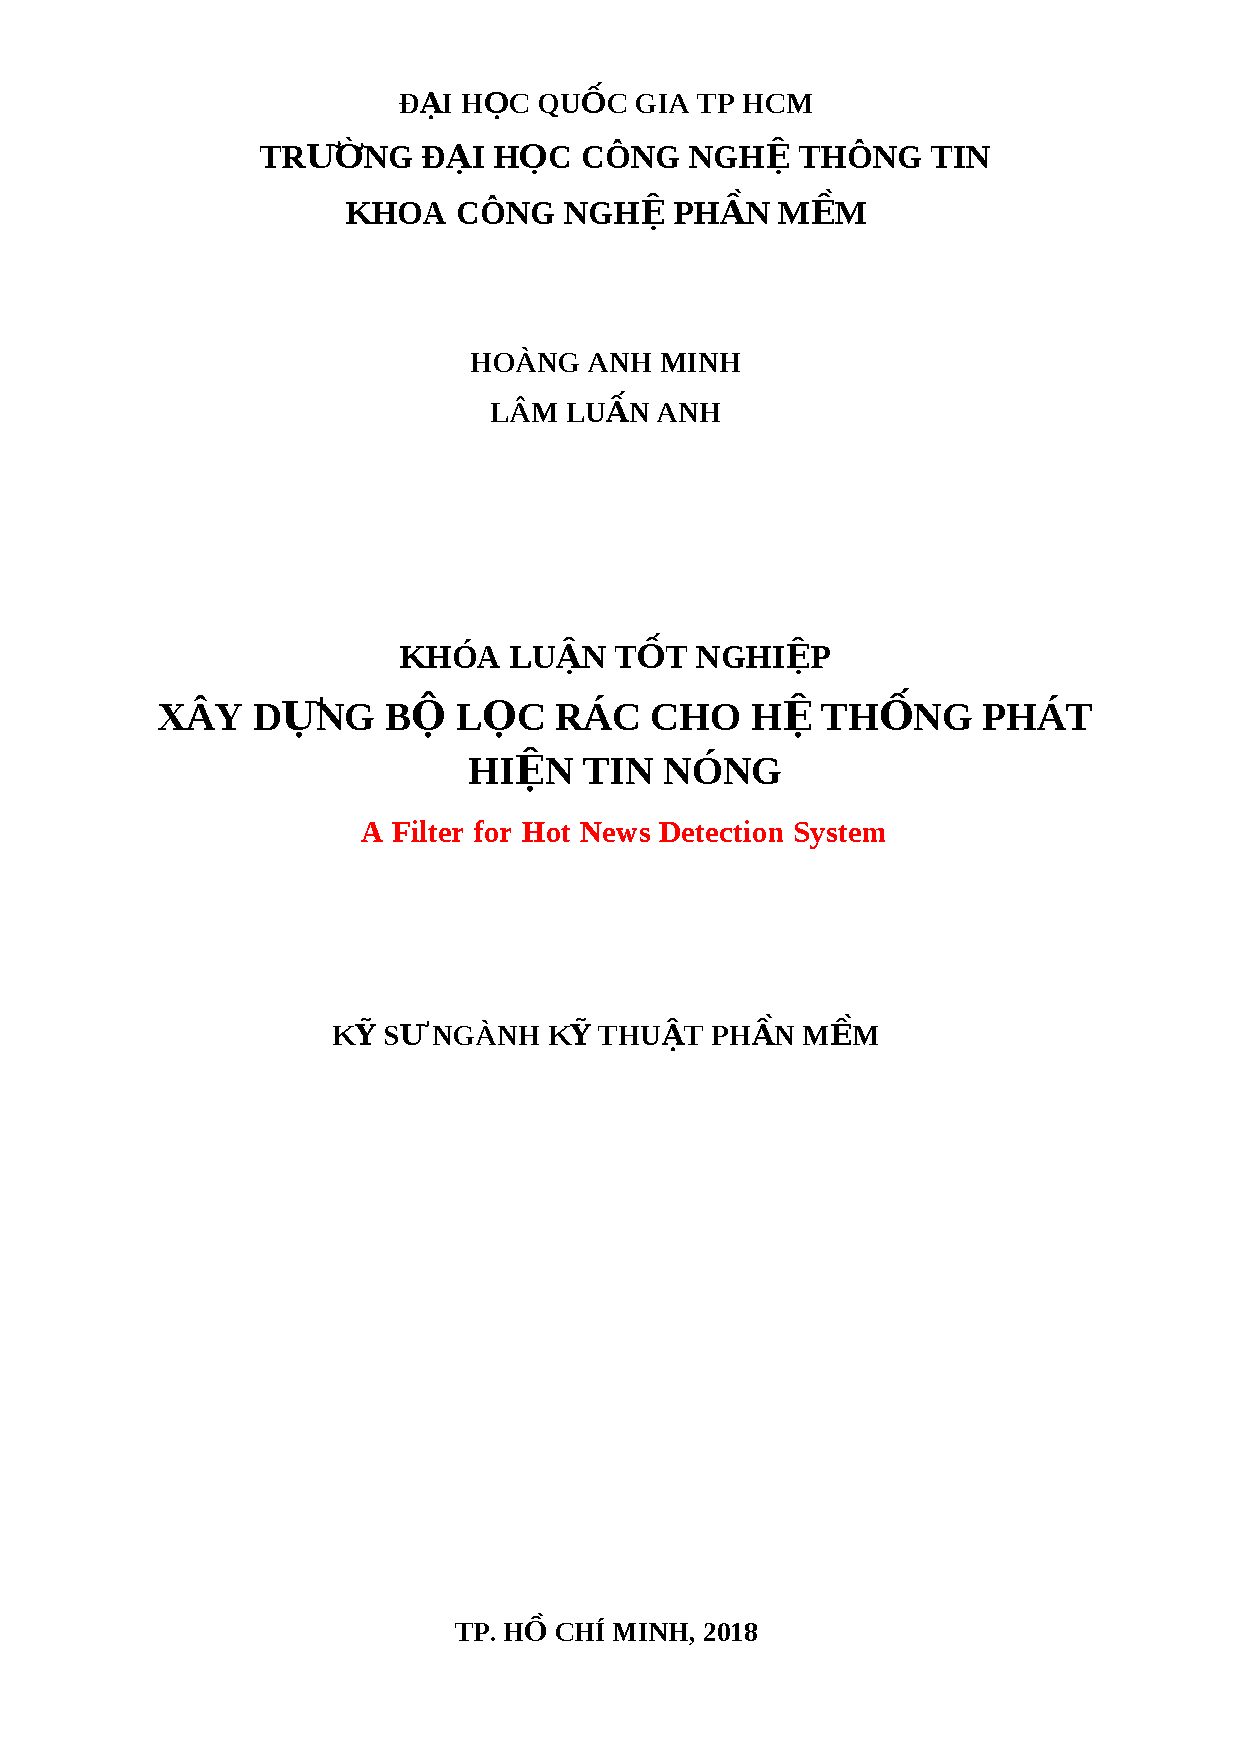
\includepdf[pages=-, scale=0.99]{BiaKhoaLuan.pdf}
\setcounter{secnumdepth}{3}
\setcounter{tocdepth}{3}

\frontmatter % book mode only
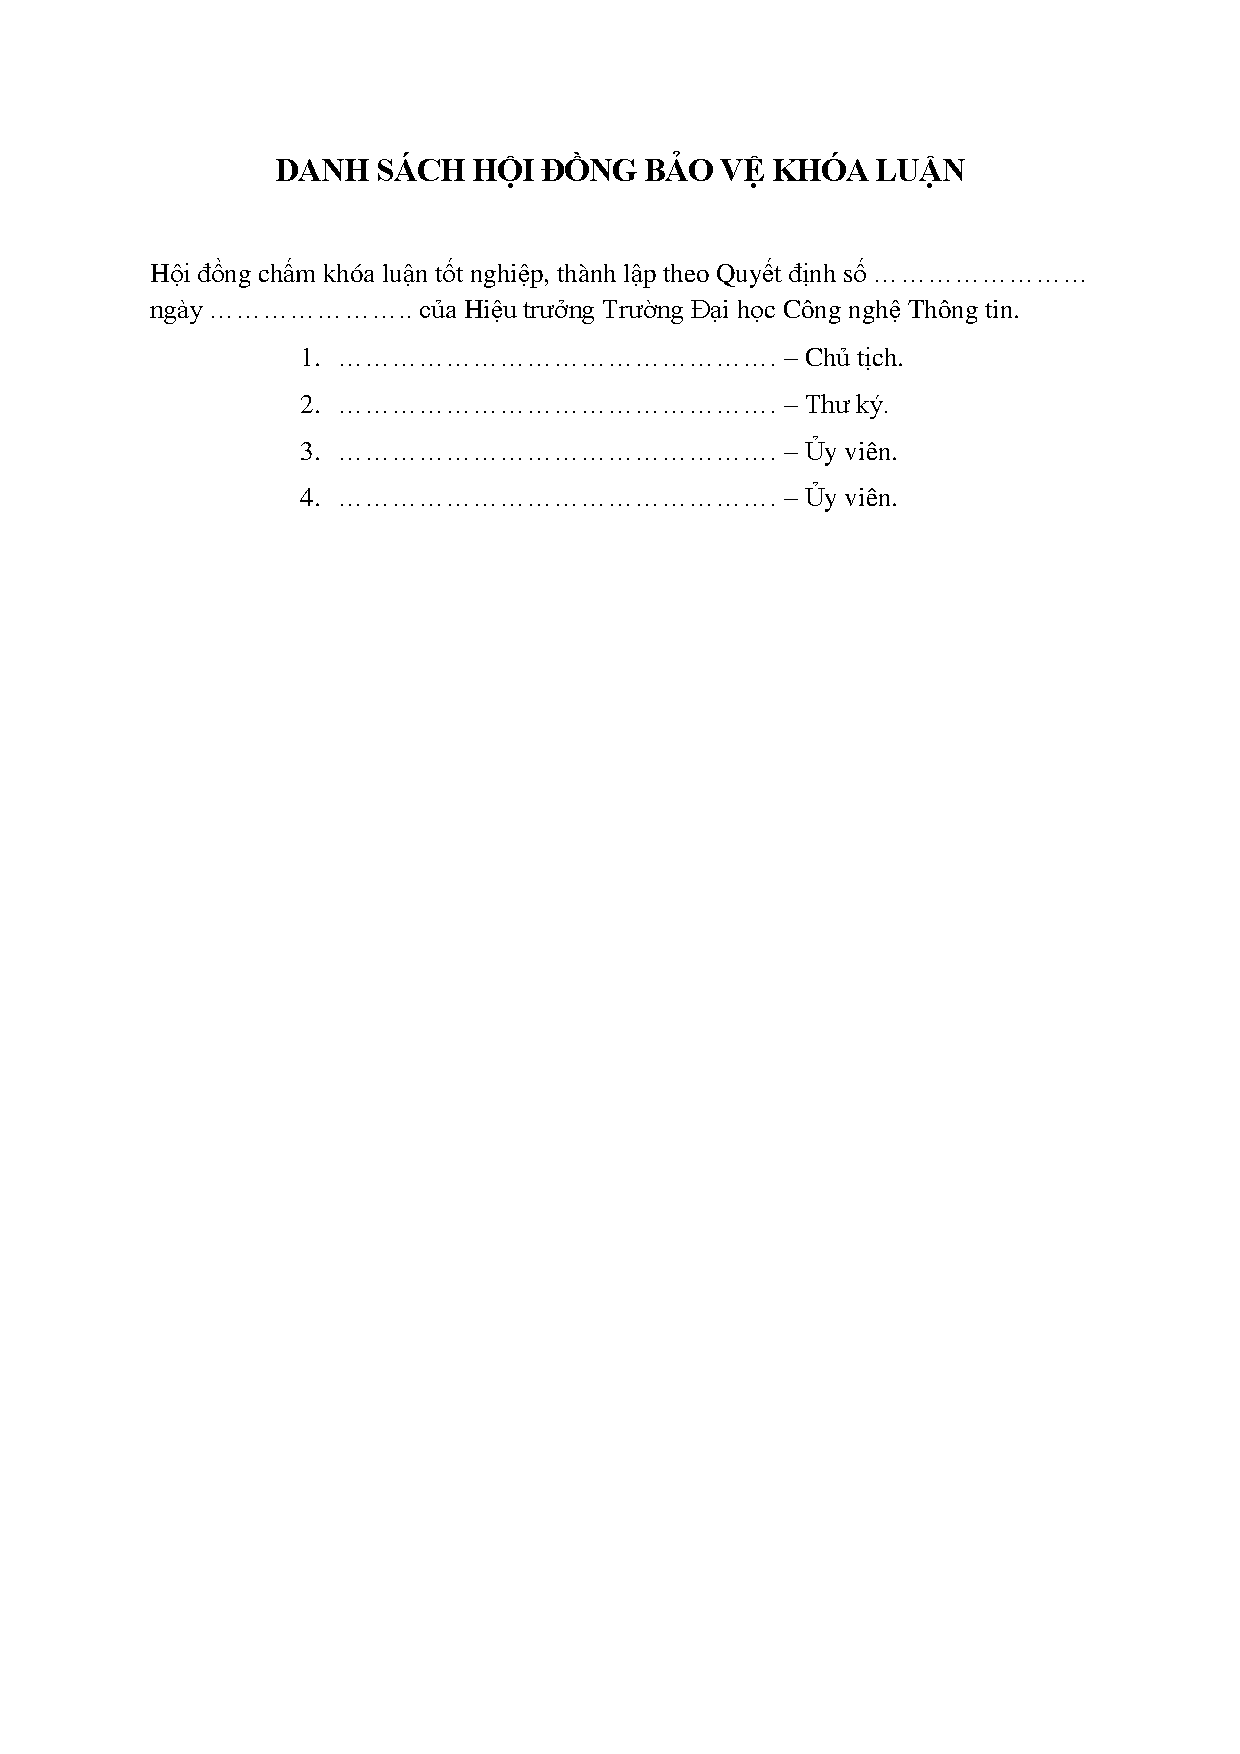
\includepdf{General/danhsachhoidong.pdf}
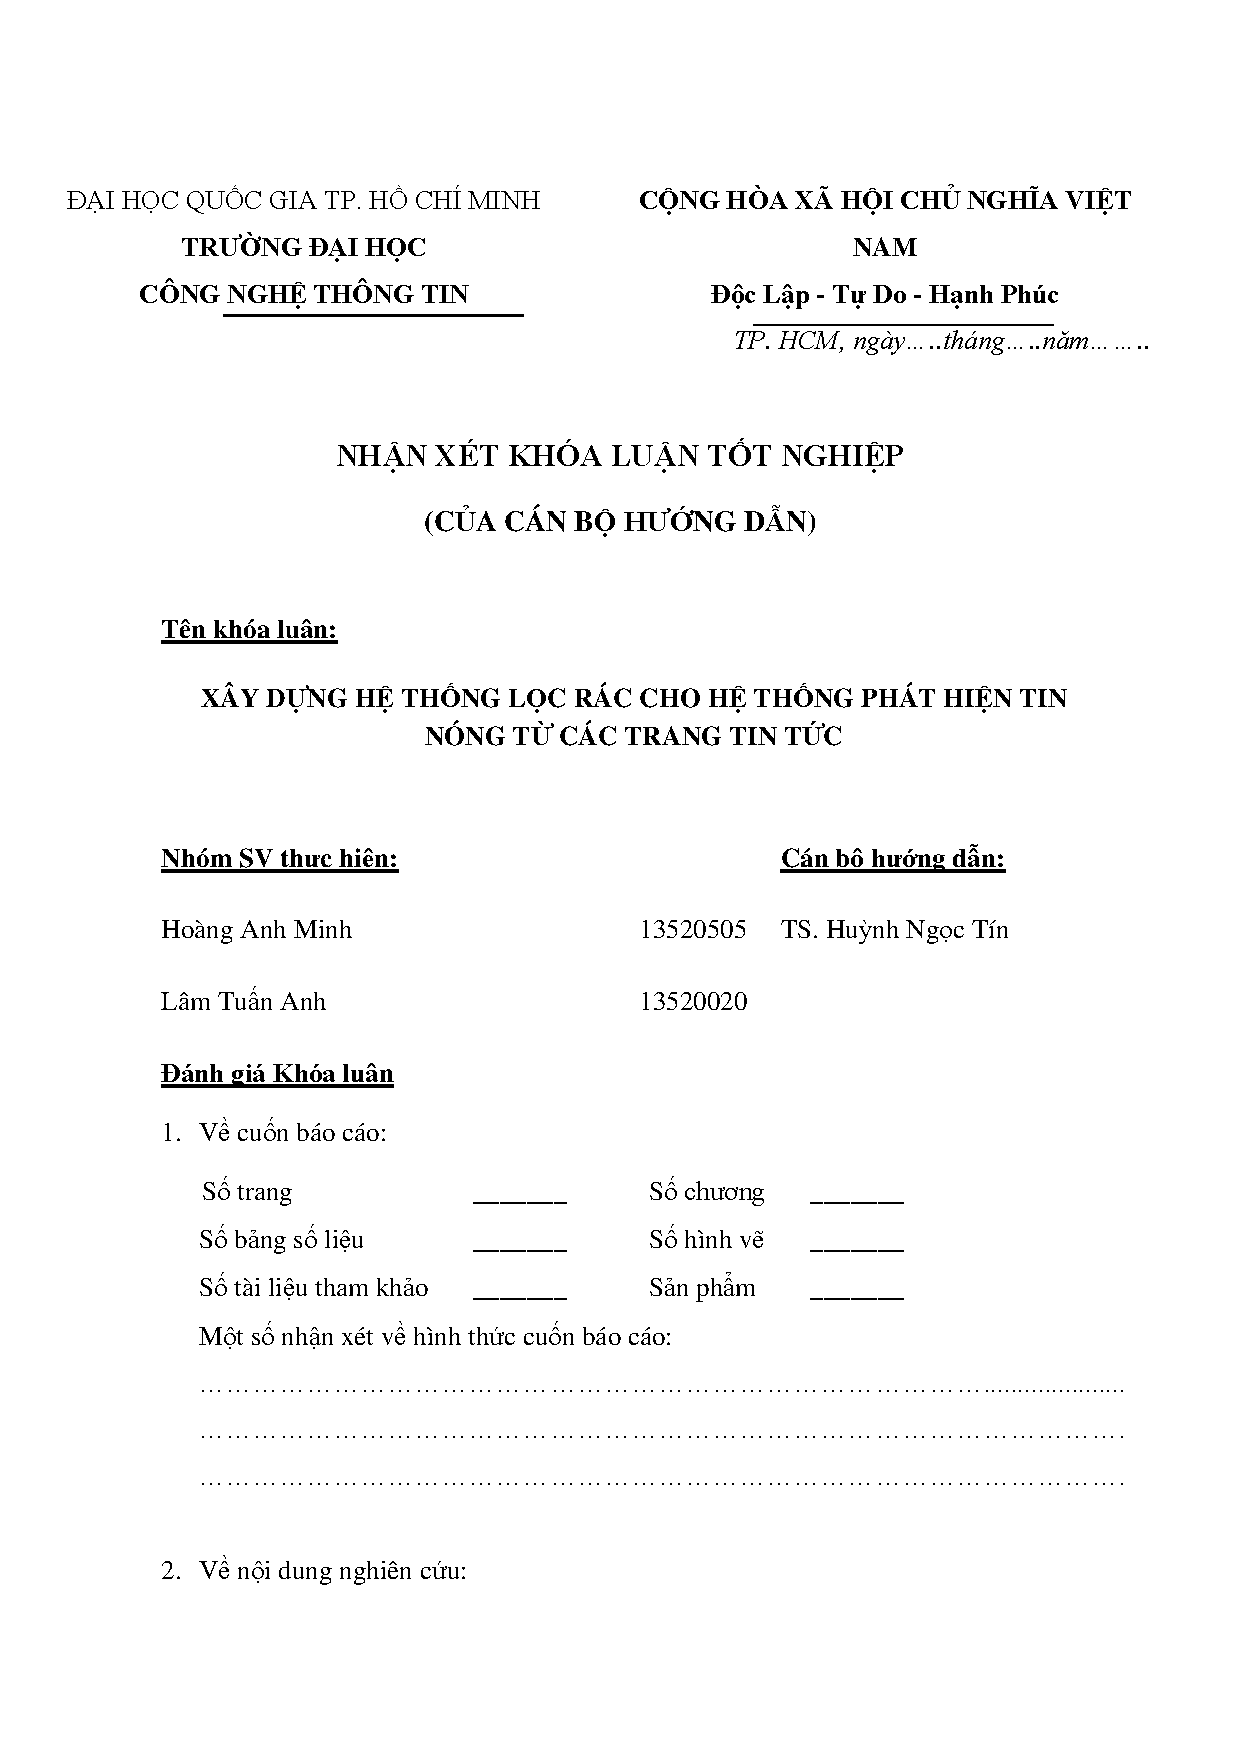
\includepdf{General/nhanxetCBHD.pdf}
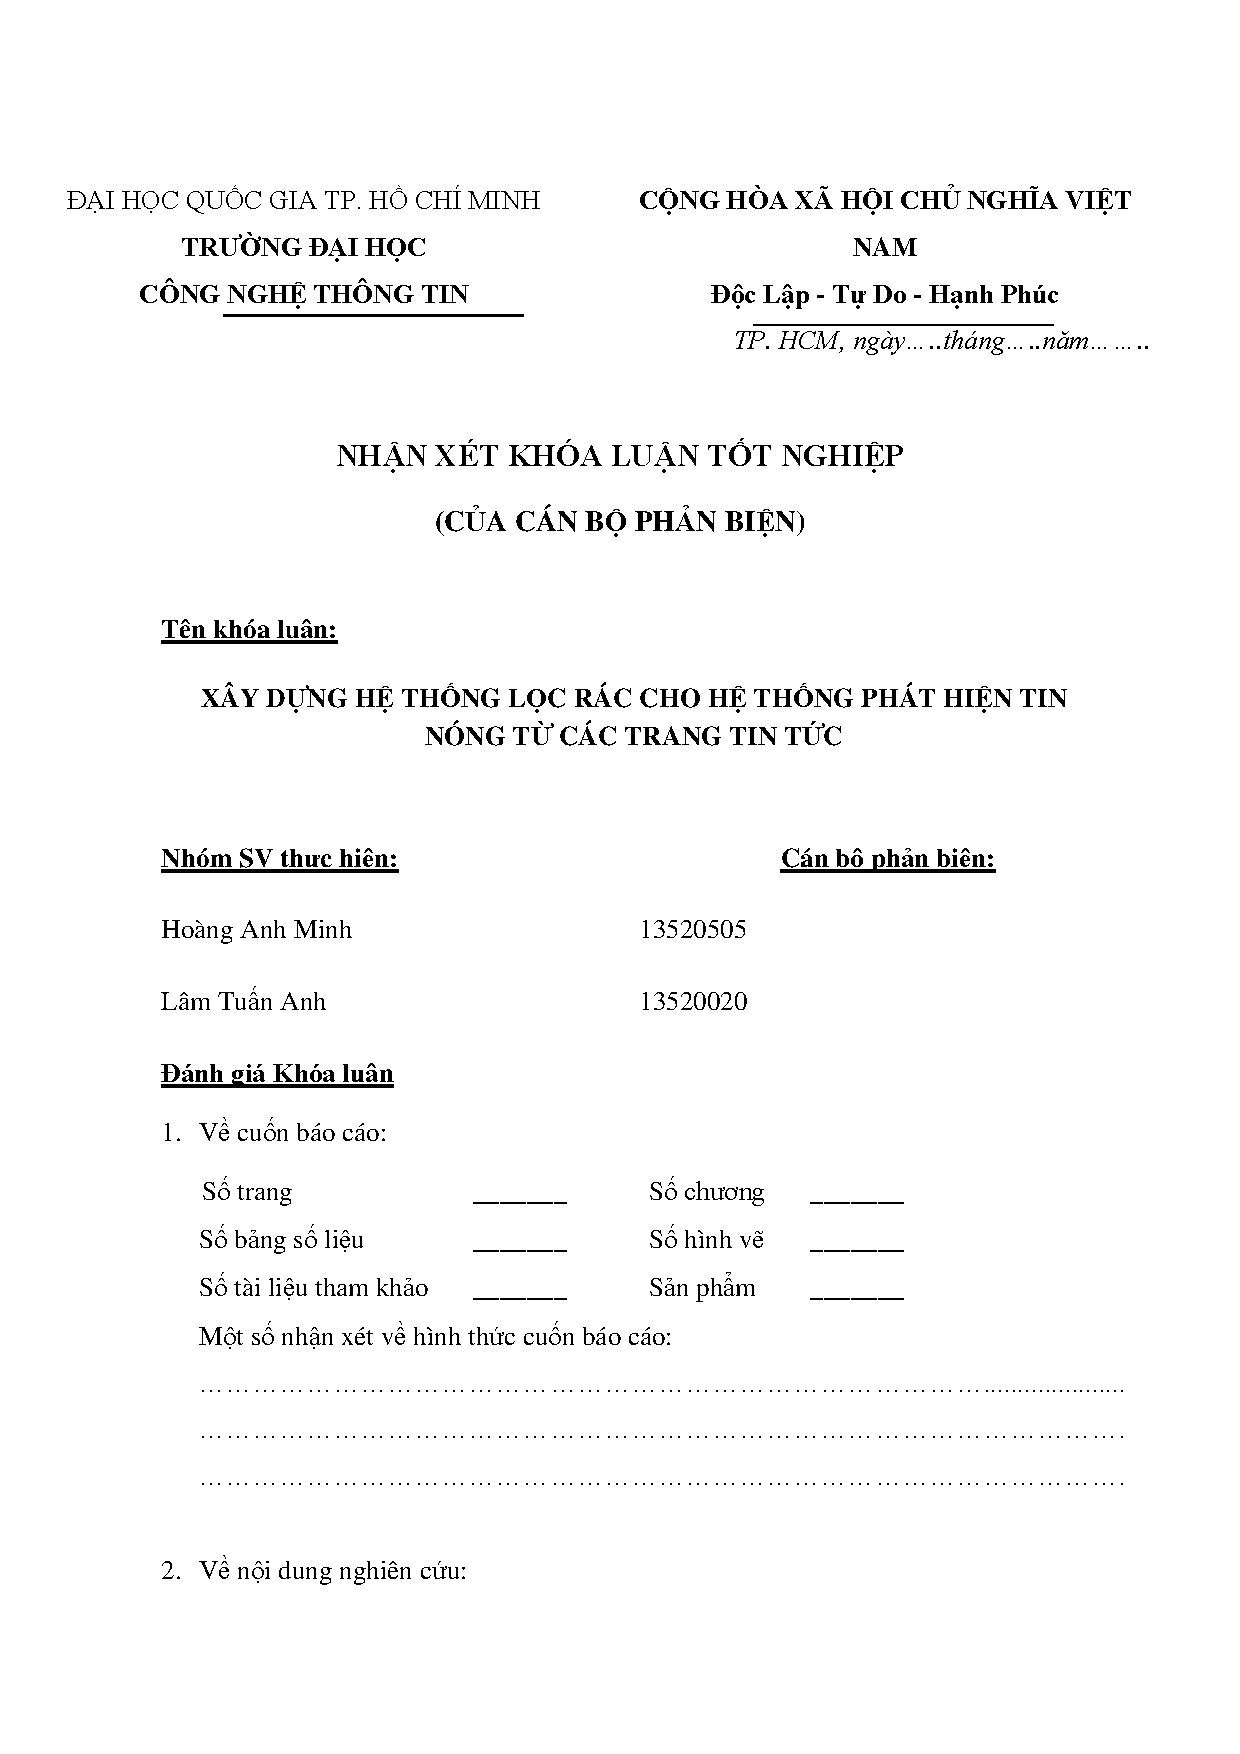
\includepdf{General/nhanxetCBPB.pdf}
\begin{acknowledgements} 

Trước tiên, em xin gửi lời cảm ơn chân thành đến TS. Huỳnh Ngọc Tín, người đã tận tình giúp đỡ, trực tiếp chỉ bảo, hướng dẫn em trong suốt quá trình thực hiện khóa luận tốt nghiệp này. Những kinh nghiệm, lời nhận xét và chia sẻ của thầy truyền đạt cho em thật sự rất quý báu và ý nghĩa.

Em cũng gửi lời cảm ơn đến quý thầy cô đang công tác tại Trường Đại học Công Nghệ Thông Tin nói chung và Khoa Khoa học máy tính nói riêng đã dạy dỗ, truyền đạt những kiến thức, kinh nghiệm vô cùng quý báu, giúp em vận dụng trong quá trình thực tập.

%Trong quá trình thực tập, vì thời và lượng kiến thức còn hạn hẹp nên chắc chắn không thể tránh khỏi những thiếu sót, em rất mong nhận được sự góp ý của Thầy cũng như các giáo viên khác đang làm việc tại trường Đại học Công Nghệ Thông Tin có thể hoàn thiện hơn nữa bài báo cáo của mình.
Ngoài ra, xin cảm ơn sự hỗ trợ quý giá của các bạn trong nhóm AdTech tại công ty VCCorp trong quá trình xây dựng hệ thống.

Cuối cùng, em xin chúc thầy luôn mạnh khỏe và đạt nhiều thành công trong cuộc sống.


Tp. HCM, tháng 12 năm 2017\\
Sinh viên thực hiện \\
Hoàng Anh Minh \\
Lâm Tuấn Anh

\end{acknowledgements}
  


\tableofcontents
\def\baselinestretch{1}
\pagestyle{fancy}
    \lhead{}    \chead{}         	\rhead{}
    \lfoot{}    \cfoot{\thepage}	\rfoot{}
    \renewcommand{\headrulewidth}{0.4pt}
    \renewcommand{\footrulewidth}{0.4pt}

\chapter*{\begin{center}Danh mục các ký hiệu, thuật ngữ và chữ viết tắt \end{center}}
\addcontentsline{toc}{chapter}{Danh mục các ký hiệu, thuật ngữ và chữ viết tắt}
\begin{tabular}{p{6.0cm} p{7.5cm}}
	Topic Detection and Tracking & : Phát hiện và theo dõi sự kiện\\
	First Story & : Bài viết đầu tiên về một sự kiện\\
	First Story Detection & : Phát hiện bài viết đầu tiên\\
	Nearest Neighbor Search & : tìm láng giềng gần nhất\\
	Locality Sensitive Hashing & : thuật toán Locality Sensitive Hashing\\
	Document & : một bài viết/điểm dữ liệu trong hệ thống\\
	Tweet & : một bài đăng bởi bất kỳ người dùng nào trên Twitter\\
	Merge Threshold & : Giá trị ngưỡng dùng khi xét hai document có đủ tương đồng để gom vào một cụm hay không\\
\end{tabular}

%\begin{center}
\listoftables  
\newpage
\listoffigures
%\end{center}
%\newpage
\mainmatter
\renewcommand\thefigure{0.\arabic{figure}} 
\setcounter{figure}{0}
\pagestyle{fancy}
    \lhead{}    \chead{}         	\rhead{}
    \lfoot{}    \cfoot{\thepage}	\rfoot{}
    \renewcommand{\headrulewidth}{0.4pt}
    \renewcommand{\footrulewidth}{0.4pt}

\chapter*{\centering TÓM TẮT KHÓA LUẬN}
\addcontentsline{toc}{chapter}{TÓM TẮT KHÓA LUẬN}
 
\ifpdf
    \graphicspath{{Abstract/AbstractFigs/PNG/}{Abstract/AbstractFigs/PDF/}{Abstract/AbstractFigs/}}
\else
    \graphicspath{{Abstract/AbstractFigs/EPS/}{Abstract/AbstractFigs/}}
\fi

Cùng với sự phát triển nhanh chóng của internet là sự tăng trưởng mạnh mẽ của ngành truyền thông báo chí. Cụ thể, tính đến ngày 31/12/2015, cả nước Việt Nam có 105 cơ quan báo điện tử, 207 trang thông tin điện tử tổng hợp của các cơ quan báo chí \footnote{http://mic.gov.vn/Pages/TinTuc/116095/Tinh-hinh-phat-trien-linh-vuc-bao-chi-va-phat-thanh-truyen-hinh-nam-2015.html}, và cứ mỗi giờ có khoảng 2,118 bài được đăng trên các trang báo mạng Việt Nam \footnote{Theo thống kê từ dữ liệu thu thập bởi công ty VCCorp tính đến tháng 7/2017.}. Cùng với sự tăng trưởng lớn về thông tin là nhu cầu phân tích và xử lý các thông tin đó để phục vụ cho nhiều mục tích khác nhau, và ngày nay nhiều doanh nghiệp đã và đang xây dựng các hệ thống phân tích dữ liệu tin tức để phục vụ tốt hơn cho người dùng và biên tập viên. 

Việc phân tích dữ liệu tin tức đòi hỏi hệ thống phải thu thập dữ liệu từ nhiều website tin tức khác nhau để có được một nguồn dữ liệu đa dạng, phong phú và đủ lớn. Tuy nhiên, dữ liệu thu thập từ các website có bản chất không phù hợp với mục đích của hệ thống phân tích có thể gây ra nhiễu và khiến cho kết quả phân tích, xử lý không chính xác. Do đó, việc sàn lọc dữ liệu thu thập được trước khi đưa vào phân tích và xử lý là cần thiết. 

Hiểu được nhu cầu trên, chúng em thực hiện khóa luận này với mục tiêu xây dựng một hệ thống lọc "rác" cho dữ liệu tin tức từ các nguồn báo chính thống Việt Nam, cụ thể là lọc "rác" cho hệ thống "Phát hiện tin nóng". 

Trong phạm vi của khóa luận, chúng em đã nghiên cứu một số thuật toán phân lớp: SVM, Naive Bayes, J48.

Sau quá trình thực hiện, đề tài khóa luận thu thập được các kết quả như sau:
	\begin{itemize}
		\item Thu thập bộ dữ liệu gồm các bài đăng trên các website tin tức Việt Nam.
		\item Đánh giá và so sánh các thuật toán: SVM, Naive Bayes, J48.
		\item Xây dựng được hệ thống lọc rác cho hệ thống phát hiện tin nóng.
	\end{itemize}


%============================
 
%Đứng trước khối lượng thông tin khổng lồ và ngày càng gia tăng với tốc độ chóng mặt nhờ sự phát triển của công nghệ số, các biên tập viên, nhà báo gặp phải nhiều khó khăn trong việc làm sao lựa chọn được thông tin đúng, phù hợp với từng lĩnh vực. Điều này đòi hỏi những người đưa tin phải dành thêm rất nhiều công sức, nguồn lực cho việc tìm kiếm, sàng lọc các nguồn tin, cũng như rất nhiều thời gian để kiểm chứng độ tin cậy của các tin đó.

%Khóa luận này được thực hiện nhằm tìm hiểu các phương pháp máy học áp dụng trong bài toán phát hiện tin nóng, với phạm vi là các bài viết từ mạng xã hội Twitter. Đồng thời xây dựng một hệ thống có khả năng nhận biết các sự kiện đáng chú ý vừa xảy ra, và thông báo cho người dùng một cách sớm nhất có thể.
\renewcommand\thefigure{1.\arabic{figure}} 
\setcounter{figure}{0}
\chapter{MỞ ĐẦU}
\ifpdf
    \graphicspath{{Chapter1/Chapter1Figs/PNG/}{Chapter1/Chapter1Figs/PDF/}{Chapter1/Chapter1Figs/}}
\else
    \graphicspath{{Chapter1/Chapter1Figs/EPS/}{Chapter1/Chapter1Figs/}}
\fi

\section{Dẫn nhập}
Trong thời đại bùng bổ về thông tin, báo chí điện tử là một trong những nguồn thông tin lớn và quan trọng cần được khai thác và phân tích một cách hiệu quả. Hệ thống phát hiện tin nóng hiện đang được triển khai và hoạt động tại VCCorp là một trong các hệ thống phân tích và xử lý dữ liệu tin tức, được phát triển nhằm mục đích xác định tin nóng từ các trang báo điện tử Việt Nam. Tuy nhiên, sự đa dạng và phong phú của nguồn tin dẫn đến việc bản chất của nhiều bài thu thập được không phù hợp với mục tiêu của hệ thống. Những bài đó, đối với hệ thống, được hiểu là "rác". Số lượng "rác" lớn sẽ gây nhiễu và làm cho việc phân tích và xử lý trở nên kém chính xác. Một cơ chế lọc rác hiệu quả sẽ giúp cải thiện độ chính xác cũng như giảm tải  cho hệ thống từ việc phân tích và xử lý các dữ liệu không có giá trị sử dụng.

Bài toán đặt ra là làm thể nào để có thể lọc "rác" trong quá trình thu thập tin tức một các chính xác. Với nhu cầu và điều kiện thuận lời từ công ty VCCorp, khóa luận này hướng đến việc xây dựng một hệ thống có khả năng lọc "rác" để tăng hiệu quả cho hệ thống phát hiện tin nóng và giúp đánh giá độ đáng tin cậy của các nguồn tin.

\section{Mục tiêu đề tài}
	\begin{itemize}
		\item Tìm hiểu và đánh giá các thuật toán phân lớp cho việc lọc rác dữ liệu tin tức
		\item Xây dựng hệ thống lọc rác áp dụng các thuật toán phân lớp.
	\end{itemize}

\section{Nội dung thực hiện}
	\begin{itemize}
		\item Tìm hiểu bài toán phân loại tin tức, tìm hiểu các phương pháp và các hướng tiếp cận
		\item Thử nghiệm đánh giá các phương pháp đã tìm hiểu:
		\begin{itemize}
			\item Thu thập dữ liệu tin tức từ cơ sở dữ liệu của công ty VCCorp.
			\item Tiến hành một số thống kê trên dữ liệu thu thập được.
			\item Huấn luyện và so sánh các thuật toán phân lớp: Naive Bayes, SVM, J48.
		\end{itemize}
	
		\item Xây dựng hệ thống:
		\begin{itemize}
			\item Tìm hiểu về MongoDB, framework Struts 2, thư viện Apache Lucene, Weka, LibSVM.
			\item Xây dựng kiến trúc hệ thống.
			\item Thiết kế chức năng, giao diện hệ thống.
			\item Cài đặt hệ thống.
		\end{itemize}
		
	\end{itemize}

\section{Phạm vi đề tài}
\begin{itemize}
	\item Nguồn dữ liệu: các bài viết từ báo chính thống Việt Nam.
	\item Ngôn ngữ: tiếng Việt.
	\item Các thuật toán tìm hiểu: Naive Bayes, SVM, J48
\end{itemize}

\section{Cấu trúc báo cáo}
Luận văn được bố cục thành chương mục như sau:
\begin{itemize}
	\item \textbf{Chương 1}: Mở đầu: Giới thiệu về đề tài.
	\item \textbf{Chương 2}: Bài toán lọc rác và các phương pháp tiếp cận phổ biến: Trình bày cơ sở lý thuyết, các khái niệm, phương pháp tiếp cận liên quan đến bài toán lọc rác.
	\item \textbf{Chương 3}: Hiện thực hệ thống lọc rác: Trình bày về kiến trúc, cài đặt hệ thống phát hiện tin nóng.
	\item \textbf{Chương 4}: Thực nghiệm và đánh giá: Trình bày về bộ dữ liệu thu thập được, đánh giá và so sánh các thuật toán.
	\item \textbf{Mục Tài liệu tham khảo}
	\item \textbf{Phụ lục. Giới thiệu về thư viện Apache Lucene}
\end{itemize}

\renewcommand\thefigure{2.\arabic{figure}} 
\setcounter{figure}{0}
\chapter{BÀI TOÁN PHÁT HIỆN TIN NÓNG VÀ CÁC PHƯƠNG PHÁP TIẾP CẬN PHỔ BIẾN}
\ifpdf
    \graphicspath{{Chapter2/Chapter2Figs/PNG/}{Chapter2/Chapter2Figs/PDF/}{Chapter2/Chapter2Figs/}}
\else
    \graphicspath{{Chapter2/Chapter2Figs/EPS/}{Chapter2/Chapter2Figs/}}
\fi

\section{Mở đầu}
Chương này sẽ giới thiệu bài toán phát hiện và theo dõi tin tức. Trình bày cơ sở lý thuyết và phát biểu bài toán phát hiện tin nóng. Cuối cùng trình bày một số phương pháp tiếp cận bài toán phát hiện tin nóng và các kiến thức liên quan.
\section{Giới thiệu bài toán} %Topic Detection and Tracking}
	\subsection{Các khái niệm cơ bản}
	Để có thể xác định khái niệm tin nóng, trước hết ta cần xem xét định nghĩa của "sự kiện" và "mẩu tin". Fiscus và Doddington \cite{Fiscus:TDTDefinition} đã tóm tắt định nghĩa về event và story như sau:
	\begin{itemize}
		\item \textit{Sự kiện (event)} là một sự việc bất kì, xảy ra tại một địa điểm cụ thể vào thời điểm xác định, cùng với những điều kiện dẫn đến nó và các hậu quả kéo theo.
		
		\item \textit{Mẩu tin (story)} là một bài viết liên quan đến một chủ đề nhất định. Có ít nhất 2 câu trần thuật độc lập với nhau.
	\end{itemize}
	
	Dựa trên quan điểm trên, ta định nghĩa tin nóng như sau:
	
	\textbf{Định nghĩa:} Tin nóng là những tin viết về một sự kiện mới xảy ra, có tính thời sự, có tầm ảnh hưởng rộng, thu hút được sự chú ý, quan tâm của cộng đồng.

%
	\subsection{Bài toán Topic Detection and Tracking}
	Topic Detection and Tracking (TDT) là một dự án bao quát được khởi xướng từ năm 1996, với mục tiêu nghiên cứu, phát triển công nghệ cho việc lưu trữ, tổ chức, tìm kiếm dữ liệu từ các nguồn \textit{tin tức} \cite{Fiscus:TDTDefinition}.
	
	Nhiệm vụ của TDT là xử lý luồng dữ liệu văn bản liên tục (từ báo chí, từ đài phát thanh, đài truyền hình thông qua các bộ chuyển giọng nói thành văn bản), từ đó theo dõi và phát hiện được các sự kiện đang diễn ra, cũng như tổ chức các bài viết thành những nhóm cùng bàn về một sự kiện nào đó.
	
	Theo Fiscus và Doddington \cite{Fiscus:TDTDefinition}, TDT được chia làm 5 tác vụ chính: 
		\begin{itemize}
			\item Story segmentation: phân đoạn dữ liệu từ đài phát thanh thành những mẩu tin riêng biệt.
			\item Topic detection: Gom nhóm các bài viết theo sự kiện, chủ đề chúng đề cập tới.
			\item Topic tracking: Theo dõi những chuyển biến của sự kiện đã diễn ra.
			\item First story detection: Phát hiện tin tức đầu tiên nói về sự kiện vừa xảy ra.
			\item Link detection: Xác định xem một cặp bài viết ngẫu nhiên có đang đề cập về cùng sự kiện không.
		\end{itemize}

	\subsection{Bài toán phát hiện tin nóng}
	Bài toán phát hiện tin nóng có thể xem là sự kết hợp giữa hai bài toán Topic Detection và First Story Detection (FSD) của TDT. Theo James Allan \cite{Allan:2002:ITD:772260.772262}, bài toán First Story Detection, hay còn gọi là New Event Detection, được đặt ra với mục tiêu phát hiện các tin tức, bài viết đầu tiên trên báo chí về các sự kiện vừa xảy ra, chưa từng được báo cáo trước đó. Ví dụ như bài viết đầu tiên đưa thông tin về một vụ tai nạn, khủng bố, hay một vụ scandal chính trị nào đó. Một hệ thống có khả năng phát hiện các first story có thể cung cấp thông tin hữu ích cho các nhà phân tích, các biên tập viên báo chí một cách nhanh chóng, kịp thời.
	
	Đối với bài toán Topic Detection, nhiệm vụ chính là gom các bài viết về cùng một sự kiện thành từng cụm, mỗi cụm là đại diện cho một sự kiện cụ thể nào đó. Do tính chất của bài toán, ta không được biết trước số lượng sự kiện (số cụm) hay nội dung từng sự kiện như thế nào, điều này hoàn toàn bởi hệ thống tự động xác định. So với FSD, bài toán này tập trung nhiều hơn vào việc nhóm được phần lớn các bài viết liên quan lại với nhau, hơn là việc phát hiện bài viết đầu tiên. Tuy nhiên trên thực tế, nhiều nhà nghiên cứu sử dụng chung một hướng giải quyết cho cả 2 bài toán này \cite{Allan:2002:ITD:772260.772262}.
	
	Ngoài nguồn dữ liệu từ báo đài, các bài viết từ mạng xã hội cũng là một nguồn tin có tiềm năng khai thác rất lớn. Tuy chất lượng bài viết và tính xác thực về nội dung có thể không tốt bằng các nguồn chính thống, các tin tức từ mạng xã hội thường có lợi thế về mặt tốc độ đưa tin. Một ví dụ nổi bật cho tính chất này là sự kiện Osama Bin Laden bị ám sát vào năm 2011, khi đó một người dùng là Keith Urbahn đã đưa thông tin lên Twitter nhanh hơn giới truyền thông đến 21 phút.

	\subsection{Phát biểu bài toán phát hiện tin nóng từ Twitter}
	Cho trước $D = (d_1, d_2, d_3,... d_n)$: chuỗi các bài viết từ Twitter được sắp xếp theo thứ tự thời gian.
	
	Mục tiêu của bài toán là phát hiện được các cụm tin $C = (c_1, c_2,... c_m)$, với mỗi phần tử $c_i = (d_{i1}, d_{i2},... d_{ik})$ là chuỗi các bài viết bàn về cùng một sự kiện cụ thể, và $d_{i1}$ là bài viết đầu tiên viết về sự kiện đó. Danh sách các chuỗi tin $C$  được sắp xếp theo thứ tự độ nóng giảm dần, với độ nóng được tính toán dựa trên thời gian đăng tin, tầm ảnh hưởng và mức độ quan tâm cộng đồng đối với sự kiện được đề cập.
	
%	Input: Tập bài viết theo thứ tự thời gian $D = \{d_1, d_2, d_3,... d_n\}$ từ nguồn Twitter.
%	Output: Tập cụm bài viết $C = \{c_1, c_2, c_3,... c_k\}$, có sắp xếp thứ tự độ quan trọng, mỗi cụm đại diện cho một sự kiện vừa diễn ra, và bài viết đầu tiên trong cụm là first story.
	
%\section{Biểu diễn dữ liệu bằng Vector space model và tf-idf}
\section{Thuật toán Naive Bayes}
\subsection{Giới thiệu thuật toán Naive Bayes}
	 Thuật toán Naive Bayes là một thuật toán phân lớp xác suất đơn giản dùng để tính một tập các xác suất bằng cách đếm tần suất và kết hợp của các giá trị trong một tập cho trước. Thuật toán sử dụng định luật Bayes sẽ giả định rằng tất cả các chiều(attributes) của dữ liệu là độc lập với nhau. Các giả định rằng các chiều là độc lập với nhau rất khó để có thể xuất hiện trong thực tế. Tuy nhiên giả thiết ngây ngô này lại mang lại những kết quả phân lớp tốt cho nhiều bài toán phân lớp \cite{dimitoglou2012comparison}.
\subsection{Lý thuyết Bayes}
    Định lý Bayes cho phép tính xác suất xảy ra của một sự kiện ngẫu nhiên A khi biết sự kiện liên quan B đã xảy ra. Xác suất này được ký hiệu là P(A|B), và đọc là “xác suất của A nếu có B”. Đại lượng này được gọi xác suất có điều kiện hay xác suất hậu nghiệm vì nó được rút ra từ giá trị được cho của B hoặc phụ thuộc vào giá trị đó.

	Theo định lí Bayes, xác suất xảy ra A khi biết B sẽ phụ thuộc vào 3 yếu tố:
	
	Xác suất xảy ra A của riêng nó, không quan tâm đến B. Kí hiệu là P(A) và đọc là xác suất của A. Đây được gọi là xác suất biên duyên hay xác suất tiên nghiệm, nó là “tiên nghiệm” theo nghĩa rằng nó không quan tâm đến bất kỳ thông tin nào về B.
	
	Xác suất xảy ra B của riêng nó, không quan tâm đến A. Kí hiệu là P(B) và đọc là “xác suất của B”. Đại lượng này còn gọi là hằng số chuẩn hóa (normalising constant), vì nó luôn giống nhau, không phụ thuộc vào sự kiện A đang muốn biết.
	
	Xác suất xảy ra B khi biết A xảy ra. Kí hiệu là P(B|A) và đọc là “xác suất của B nếu có A”. Đại lượng này gọi là khả năng (likelihood) xảy ra B khi biết A đã xảy ra. Chú ý không nhầm lẫn giữa khả năng xảy ra B khi biết A và xác suất xảy ra A khi biết B.
	
	Tóm lại định lý Bayes sẽ giúp ta tính ra xác suất xảy ra của một giả thuyết bằng cách thu thập các bằng chứng nhất quán hoặc không nhất quán với một giả thuyết nào đó. Khi các bằng chứng tích lũy, mức độ tin tưởng vào một giả thuyết thay đổi. Khi có đủ bằng chứng, mức độ tin tưởng này thường trở nên rất cao hoặc rất thấp, tức là xác xuất sảy ra giả thuyết sẽ thay đổi thì các bằng chứng liên quan đến nó thay đổi.
	
	Công thức của định luật Bayes được phát biểu như sau:
\begin{equation}
	P(A \mid B) = \frac{P(B \mid A) \, P(A)}{P(B)}
\end{equation}
Trong đó:
\begin{itemize}
	\item P(A|B) là  xác suất xảy ra của một sự kiện ngẫu nhiên A khi biết sự kiện liên quan B đã xảy ra.
	\item P(B|A) là xác suất xảy ra B khi biết A xảy ra
	\item P(A) là xác suất sảy ra của riêng A mà không quan tâm đến B.
	\item P(B) là xác suất xảy ra của riêng B mà không quan tâm đến A.
\end{itemize}
	Ở trên ta có thể thấy xác suất sảy ra của giả thuyết A phụ thuộc và xác suất của giả thuyết B, nhưng trong thực tế xác suất A có thể phụ thuộc vào xác suất của nhiều các giác thuyết khác có thể là B1, B2, B3 … Bn. Vậy định luật Bayes có thể được mở rộng bằng công thức sau:
\begin{equation}
	P(A \mid B) = \frac{\left(P(B_1 \mid A) \times P(B_2 \mid A) \times P(B_3 \mid A)... \times P(B_n \mid A)\right) \times P(A)}{P(B_1) \times P(B_2) \times P(B_3)... \times P(B_n)}
\end{equation}
\subsection{Naive Bayes Classifier}
	Xét bài toán classification với C classes 1,2,…,C. Giả sử có một điểm dữ liệu $x \in \mathbb{R}^d $. Hãy tính xác suất để điểm dữ liệu này rơi vào class c. Nói cách khác, hãy tính:
\begin{equation}
	p(y = c \mid x)
\end{equation}
	hoặc viết gọn là $p(c \mid x)$
	Tức tính xác suất để đầu ra là class c biết rằng đầu vào là vector x.
	Biểu thức này, nếu tính được, sẽ giúp chúng ta xác định được xác suất để điểm dữ liệu rơi vào mỗi class. Từ đó có thể giúp xác định class của điểm dữ liệu đó bằng cách chọn ra class có xác suất cao nhất:
\begin{equation}
	c = \arg\max_{c \in \left\{1,..,C \right\}} p(c \mid x)
\end{equation}
Biểu thức (2) thường khó được tính trực tiếp. Thay vào đó, quy tắc Bayes thường được sử dụng:
\begin{align}
	c = \arg\max_{c } p(c \mid x) \label{NB1} \\
	  = \arg\max_{c }\frac{p(x \mid c) p(c)}{p(x)} \label{NB2} \\
	  = \arg\max_{c } p(x \mid c) p(c) \label{NB3}
\end{align}
	Từ \eqref{NB1} sang \eqref{NB2} là vì quy tắc Bayes. Từ \eqref{NB2} sang \eqref{NB3} là vì mẫu số p(x) không phụ thuộc vào c.
	Tiếp tục xét biểu thức \eqref{NB3}, p(c) có thể được hiểu là xác suất để một điểm rơi vào class c. Giá trị này có thể được tính bằng MLE, tức tỉ lệ số điểm dữ liệu trong tập training rơi vào class này chia cho tổng số lượng dữ liệu trong tập traing; hoặc cũng có thể được đánh giá bằng MAP estimation. Trường hợp thứ nhất thường được sử dụng nhiều hơn.
	
	Thành phần còn lại p(x|c), tức phân phối của các điểm dữ liệu trong class c, thường rất khó tính toán vì x là một biến ngẫu nhiên nhiều chiều, cần rất rất nhiều dữ liệu training để có thể xây dựng được phân phối đó. Để giúp cho việc tính toán được đơn giản, người ta thường giả sử một cách đơn giản nhất rằng các thành phần của biến ngẫu nhiên x là độc lập với nhau, nếu biết c (given c..) Tức là:
\begin{equation}
	p(x \mid c) = p(x_1,x_2,...,x_d \mid c) = \displaystyle \prod_{i=1}^d p(x_i \mid c)
\end{equation}
	Khi một dữ liệu mới được thêm vào, Naive Bayes sẽ xác định lớp của điểm dữ liệu x bởi:
\begin{equation}
	c = \arg\max_{c \in \left\{ 1,...,C\right\}} p(c) \prod_{i=1}^{d}p(x_i \mid c) 
	\label{NB4}
\end{equation}
Khi d lớn và các xác suất nhỏ, biểu thức ở vế phải của \ref{NB4} sẽ là một số rất nhỏ, khi tính toán có thể gặp sai số. Để giải quyết việc này, \ref{NB4} thường được viết lại dưới dạng tương đương bằng cách lấy log của vế phải:
 \begin{equation}
 	c = \arg\max_{c \in \left\{ 1,...,C\right\}} = \log(p(c) + \sum_{i=1}^{d}\log(p(x_i \mid c)))
 \end{equation}
	Việc này không ảnh hưởng tới kết quả vì log là một hàm đồng biến trên tập các số dương.
	 
	Mặc dù giả thiết mà Naive Bayes Classifiers sử dụng là quá phi thực tế, chúng vẫn hoạt động khá hiệu quả trong nhiều bài toán thực tế, đặc biệt là trong các bài toán phân loại văn bản, ví dụ như lọc tin nhắn rác hay lọc email spam. Trong phần sau của bài viết, chúng ta cùng xây dựng một bộ lọc email spam tiếng Anh đơn giản.
	 
	Cả việc training và test của NBC là cực kỳ nhanh khi so với các phương pháp classification phức tạp khác. Việc giả sử các thành phần trong dữ liệu là độc lập với nhau, nếu biết class, khiến cho việc tính toán mỗi phân phối p(xi|c) trở nên cực kỳ nhanh.
	 
	Mỗi giá trị p(c),c=1,2,…,C có thể được xác định như là tần suất xuất hiện của class c trong training data.
	 
	Việc tính toán p(xi|c) phụ thuộc vào loại dữ liệu. Có ba loại được sử dụng phổ biến là: Gaussian Naive Bayes, Multinomial Naive Bayes, và Bernoulli Naive.
\subsection{Một số phân phối thường dùng}
	\subsubsection{Gaussian Naive Bayes}
		Mô hình này được sử dụng chủ yếu trong loại dữ liệu mà các thành phần là các biến liên tục. Với mỗi chiều dữ liệu i và một class c, xi tuân theo một phân phối chuẩn có kỳ vọng $ \mu_{ci} $ và phương sai $\sigma_{ci}^2$:
	\begin{equation}
		p(x_i \mid c) = p(x_i \mid \mu_{ci}, \sigma_{ci}^2)=\frac{1}{\sqrt{2\pi\sigma_{ci}^2}}\exp(\frac{(x_i - \mu_{ci})^2}{2 \sigma_{ci}^2})  
	\end{equation}
		Trong đó, bộ tham số $\theta = { \mu_{ci}, \sigma_{ci}^2}$ được xác định bằng Maximum Likehood
	\begin{equation}
		(\mu_{ci}, \sigma_{ci}^2)=\arg\max_{\mu_{ci}, \sigma_{ci}^2}\prod_{i=1}^n p(x_i^(n) \mid \mu_{ci},\sigma_{ci}^2 )
	\end{equation}
	\subsubsection{Multinominal Naive Bayes}
	Mô hình này chủ yếu được sử dụng trong phân loại văn bản mà feature vectors được tính bằng Bags of Words. Lúc này, mỗi văn bản được biểu diễn bởi một vector có độ dài d chính là số từ trong từ điển. Giá trị của thành phần thứ i trong mỗi vector chính là số lần từ thứ i xuất hiện trong văn bản đó.
	
	Khi đó, p(xi|c) tỉ lệ với tần suất từ thứ i (hay feature thứ i cho trường hợp tổng quát) xuất hiện trong các văn bản của class c. Giá trị này có thể được tính bằng cách:
	\begin{equation}
		\lambda_{ci}=p(x_i \mid c) = \frac{N_ci}{N_c}
	\end{equation}
	Trong đó:
	\begin{itemize}
		\item $N_ci$ là tổng số lần từ thứ i xuất hiện trong các văn bản của class c, nó được tính là tổng của tất cả các thành phần thứ i của các feature vectors ứng với class c
		\item $N_c$ là tổng số từ (kể cả lặp) xuất hiện trong class c. Nói cách khác, nó bằng tổng độ dài của toàn bộ các văn bản thuộc vào class c. Có thể suy ra rằng $N_c$=$ \sum_{i=1}^d=N_ci$, từ đó =$ \sum_{i=1}^d \lambda_{ci}=1$.
	\end{itemize}
		
	Cách tính này có một hạn chế là nếu có một từ mới chưa bao giờ xuất hiện trong class c
	thì biểu thức (10) sẽ bằng 0, điều này dẫn đến vế phải của (7) bằng 0 bất kể các giá trị còn lại có lớn thế nào. Việc này sẽ dẫn đến kết quả không chính xác (xem thêm ví dụ ở mục sau).
	Để giải quyết việc này, một kỹ thuật được gọi là Laplace smoothing được áp dụng:
	\begin{equation}
		\hat{\lambda_{ci}} = \frac{N_{ci}+ \alpha}{N_c+d_\alpha}
	\end{equation}
	Với $\alpha$ là một số dương, thường bằng 1, để tránh trường hợp tử số bằng 0. Mẫu số được cộng với $d_\alpha$ để đảm bảo tổng xác suất $ \sum_{i=1}^d \hat{\lambda_{ci}}=1$.
	Như vậy, mỗi class c sẽ được mô tả bởi bộ các số dương có tổng bằng 1: $ \hat{\lambda_{c}}= \left\{\hat{\lambda_{c1}}+,...,+\hat{\lambda_{cd}}\right\}$.
	\subsubsection{Bernoulli Naive}
	Mô hình này được áp dụng cho các loại dữ liệu mà mỗi thành phần là một giá trị binary - bẳng 0 hoặc 1. Ví dụ: cũng với loại văn bản nhưng thay vì đếm tổng số lần xuất hiện của 1 từ trong văn bản, ta chỉ cần quan tâm từ đó có xuất hiện hay không.
	
	Khi đó, $p(x_i \mid c $ được tính bằng:
	\begin{equation}
		p(x_i \mid c) = p(i \mid c)x_i + 1-p(i\mid c)(1- x_i)
	\end{equation}
	với p(i|c) có thể được hiểu là xác suất từ thứ i xuất hiện trong các văn bản của class c.
	 
	\subsection{Ưu điểm thuật toán Naive Bayes}
	\subsection{Nhược điểm điểm thuật toán Naive Bayes}
	\subsection{Naive Bayes với bài toán lọc rác tin tức}
\section{Thuật toán J48}
	\subsection{Giới thiệu thuật toán J48}
		Thuật toán J48(C4.5) là một thuật toán sử dụng cây quyết định(decision tree) cho việc phân lớp. Thuật toán sẽ tạo ra môn cây nhị phân. Bằng cách sử dụng cây quyết định, cách tiếp cận này cũng thường đước sử dụng trong bài toán phân lớp. Cây quyết định sẽ được xây dựng để mô hình hóa quá trình phân lớp.
	\subsection{Lý thuyết cây quyết định}
		Cây quyết định (Decision Tree) là một cây phân cấp có cấu trúc được dùng để phân lớp các đối tượng dựa vào dãy các luật (series of rules). Các thuộc tính của đối tượng (ngoại trừ thuộc tính phân lớp – Category attribute) có thể thuộc các kiểu dữ liệu khác nhau (Binary, Nominal, ordinal, quantitative values) trong khi đó thuộc tính phân lớp phải có kiểu dữ liệu là Binary hoặc Ordinal.
		Tóm lại, cho dữ liệu về các đối tượng gồm các thuộc tính cùng với lớp (classes) của nó, cây quyết định sẽ sinh ra các luật để dự đoán lớp của các đối tượng chưa biết (unseen data)
	\subsection{Ví dụ về cây quyết định J48}
	\begin{figure}[H]
		\centering
		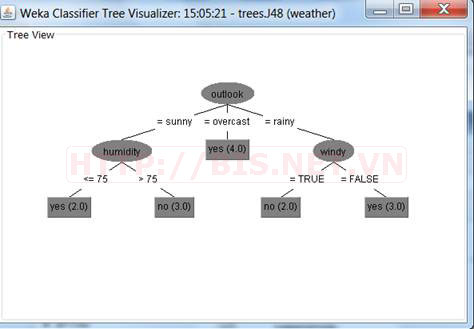
\includegraphics[width=0.9\linewidth]{Chapter2/Chapter2Figs/Decision_Tree_007}
		\caption{Ví dụ về cây quyết định}
		\label{fig:DecisionTreeExample}
	\end{figure}
\section{Tiền xử lý}
\subsection{Khái niệm}
Tiền xử lý dữ liệu là quá trình lọc và chuẩn bị dữ liệu cho quá trình phân lớp văn bản. Thường các văn bản đầu vào đa số chứa nhiều thông tin gây nhiễu và các thông tin không có giá trị như HTML tags, địa chỉ trang web, quảng cáo... Vì vậy, ở mức độ từ, nhiều từ không có ý nghĩa cho ý chung của câu.
\subsection{Vì sao phải tiền xử lý}
Giữ những từ có khả năng gây nhiễu sẽ làm tăng số chiều làm quá trình phân lớp trở nên khó hơn vì mỗi từ được xem như một chiều cần phải xem xét. Đây là lý do chúng ta cần tiền xử lý dữ liệu: để giảm nhiễu trong văn bản sẽ giúp tăng hiệu năng của bộ phân lớp(classfier) và làm giảm thời gian phân lớp.
\subsection{Một số cách tiếp cận}
Quá trình tiền xử lý dữ liệu thường sẽ gồm các bước:
\begin{itemize}
	\item Loại bỏ một số thông tin không cần thiết (Ví dụ như HTML tags,...)
	\item Loại bỏ một số dấu câu không cần thiết (khoảng trắng hoặc dấu câu)
	\item Loại bỏ stop-word: Một số từ thường xuất hiện trong văn bản nhưng không mang nhiều ý nghĩa. Thường sẽ được lưu thành một stop-word list. Ở tiếng Việt, một số stop word là(à, á, á à, ạ,....)
	\item Ghép từ một số từ ghép được ghép lại để biểu diễn cho một chiều trong phân lớp (Ví dụ máy bay sẽ ghép thành máybay hoặc máy\_bay)
\end{itemize}
\subsection{Tiền xử lý trong bài toán lọc rác tin tức}
Ở bài toán lọc rác tin tức, dữ liệu đầu vào là tin tức nên đa số thông tin gây nhiễu như quảng cáo, HTML tags đã được giảm thiểu, chúng ta chỉ cần xử lý văn bản và lọc một số thông tin gây nhiễu. Ví dụ như:
\begin{itemize}
	\item Link(URL) nếu có.
	\item Ghép từ để tăng độ chính xác (ví dụ máy bay sẽ được ghép thành máy\_bay)
	\item Loại bỏ stop-word
\end{itemize} 
\section{Các nghiên cứu liên quan}
Twitter đã thu hút sự chú ý của nhiều nhà nghiên cứu trong thời gian gần đây. Nhờ vào sự phổ biến rộng rãi trên nhiều quốc gia, cùng với vai trò là một mạng xã hội cho phép người dùng chia sẻ thông tin một cách nhanh chóng và ngắn gọn.
Jagan Sankaranarayanan và cộng sự \cite{TwiterStand:Sankaranarayanan} đã xây dựng một hệ thống xử lý tin tức trên Twitter, với tên là Twitter Stand. Hệ thống biểu diễn dữ liệu dưới dạng tf-idf, và sử dụng thuật toán phân lớp Naive Bayes để lọc bỏ các tin rác. Sau đó dùng một thuật toán online clustering để gom các tin thành từng câu chuyện.
Phuvipadawat và cộng sự \cite{SwitPhuvipadawat} đưa ra phương pháp phát hiện tin nóng trên Twitter dựa vào tiếp cận gom cụm. Các tweet được thu thập thông qua Twitter Search API với một số từ khóa (VD: "breaking news", "\#breakingnews"). Độ tương đồng giữa các bài viết được tính theo công thức dựa trên tf-idf, với các danh từ riêng, các hashtag và tên người dùng được tăng trọng số. Tác giả nhấn mạnh việc tăng trọng số như vậy giúp tăng độ chính xác của thuật toán, bởi độ dài tweet giới hạn.
\section{Giới thiệu một số độ đo khoảng cách/sự tương đồng} \label{distances}
Một thành phần tất yếu của tiếp cận gom cụm là tiêu chí, độ đo được sử dụng để định lượng sự tương đồng giữa các đối tượng. Dưới đây là một số độ đo phổ biến.
	\subsection*{Euclidean Distance}
	Euclidean Distance là độ đo khoảng cách tiêu chuẩn trong các vấn đề liên quan đến hình học, và cũng thường được sử dụng trong các bài toán gom cụm. Công thức tính Euclidean distance \cite{IntroToIR}:
		\begin{equation}
		D_{Euclidean}(\vec{x}, \vec{y}) = \sqrt{\sum_{i=1}^n (x_i-y_i)^2}
		\end{equation}
	với n là số chiều của vector biểu diễn document, $x_i$ và $y_i$ lần lượt là giá trị tọa độ thứ i của document x và y\\	
	\subsection*{Cosine Similarity}
	Cosine Similarity phản ánh góc chênh lệch giữa 2 vector, mà không cân nhắc đến độ lớn của vector. Độ đo này được áp dụng rộng rãi đối với dữ liệu văn bản. Cách tính \cite{IntroToIR}: 
		\begin{equation}
		Similarity_{Cosine}(\vec{x}, \vec{y}) = \frac {\vec{x} \cdot \vec{y}}{||\vec{x}|| \cdot ||\vec{y}||} = \frac{\sum_{i=1}^{n}x_iy_i}{\sqrt{\sum_{i=1}^{n}x_i^2} \sqrt{\sum_{i=1}^{n}y_i^2}}	
		\end{equation}
	với  $x_i$ và $y_i$ lần lượt là giá trị tọa độ thứ i của document x và y
\section{Các phương pháp tiếp cận phổ biến}
Gom cụm, gom nhóm là quá trình nhóm các đối tượng thành những nhóm/cụm/lớp, qua đó phát hiện được cấu trúc, ý nghĩa tiềm ẩn của dữ liệu. Các đối tượng trong cùng một nhóm có nhiều tính chất chung và có những tính chất khác với các đối tượng ở nhóm khác. Đây là một trong những tác vụ chính của ngành khai thác dữ liệu, và được dùng trong nhiều lĩnh vực như: máy học, nhận diện mẫu, phân tích ảnh,...
Bài toán gom cụm bao gồm nhiều phương pháp khác nhau như: phân hoạch, phân cấp, dựa trên mật độ, dựa trên mô hình,... Trong khóa luận này chỉ sử dụng đến \textit{phương pháp phân hoạch}. 	
\subsection{Thuật toán gom cụm k-láng giềng gần (k-Nearest Neighbor)}
	\subsubsection{Ý tưởng}
		%sửa lại chỉ nói về NNS thôi chứ không nói ý tưởng giải FSD?
		Hướng tiếp cận truyền thống của bài toán FSD là sử dụng phương pháp gom cụm k-láng giềng gần nhất, với k = 1 \cite{Allan00detectionsbounds}. Theo trực quan ta có thể thấy nếu một bài viết có nội dung tương tự nhiều với những bài có sẵn, thì khả năng nó là một first story rất thấp. Ngược lại, khi nội dung của một bài viết mới lạ, khác hẳn những bài viết trước đây, thì có thể xem đó là một first story.
		
		Thuật toán gom cụm này hoạt động như sau: Mỗi document mới sẽ được so sánh với tất cả các document hiện có trong hệ thống và tìm ra một document tương đồng nhất. Nếu độ tương đồng của chúng cao hơn một ngưỡng cho trước, thì document mới này sẽ được gán vào cụm của document tương đồng nhất, ngược lại tạo cụm mới và xem document mới như một first story.
		
	\subsubsection{Minh họa thuật toán}
		Giả sử ta có dữ liệu như hình vẽ. Đường tròn thể hiện ngưỡng khoảng cách để một document được xem là first story hay không, chọn ngưỡng giá trị 0.8. Ta có sẵn 4 document và 1 document mới vào hệ thống như sau:
		\begin{center}
					doc1 = (3,4,1,2)\\
				doc2 = (1,1,5,6)\\
				doc3 = (1,2,4,4)\\
				doc4 = (3,5,1,1)\\
				newDoc = (2,1,4,5)\\
		\end{center}
		\begin{table}[H]
			\centering
			\begin{tabular}{|p{1.5cm}|p{1.5cm}|p{1.5cm}|p{1.5cm}|p{1.5cm}|p{1.5cm}|}
				\hline
				& doc1 & doc2 & doc3 & doc4 & \textbf{newDoc} \\
				\hline 
				doc1 & 1 & 0.55202 & 0.6903 	& 0.973729 & 0.646058 \\
				doc2 &   & 1 		& 0.973479 	& 0.398962 & 0.984525 \\
				doc3 &   &   		& 1			& 0.575396 & 0.969572 \\
				doc4 &   &  		&  			& 1 	& 0.491473 \\
				newDoc &   &  		&  			&   	& 1 \\
				\hline
			\end{tabular}
			\caption{Độ tương đồng cosine giữa các document} \label{tab:table_1_1}
		
		\end{table}
		Ta có thể thấy document tương tự nhất của newDoc là doc2 (0.984525), lớn hơn ngưỡng cho trước (0.8), do đó newDoc được cho vào chung cụm với doc2 và không phải là một first story.
	
		\begin{figure}[H]
			\begin{center}
				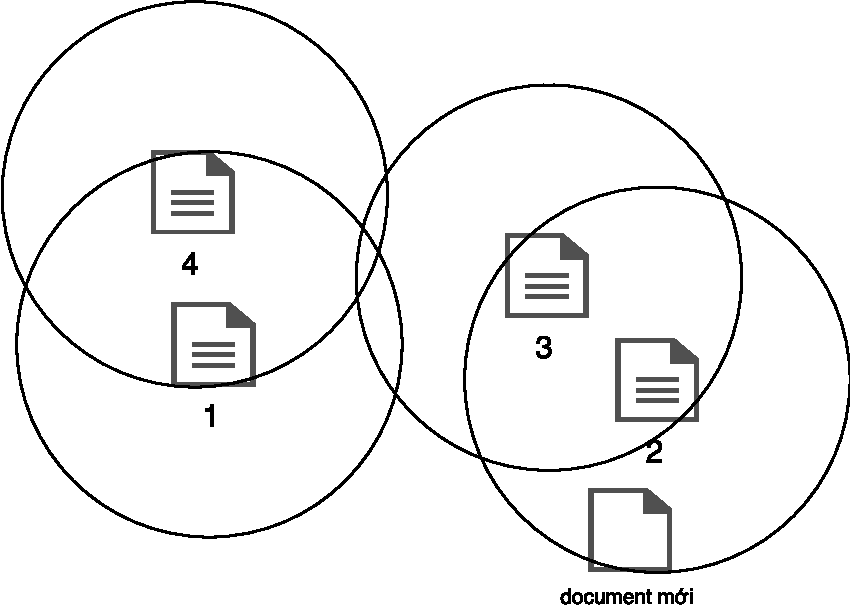
\includegraphics[width=0.9\linewidth]{NNS.pdf}
				\caption{Cách xử lý một document mới trong thuật toán Nearest Neighbor Search}
			\end{center}
		\end{figure}
		
	\subsubsection{Mã giả}
		\begin{algorithm}[H]
			\caption{Phát hiện tin nóng dựa trên k-Nearest neighbor}
			\begin{algorithmic}[1]
				\REQUIRE luồng bài viết từ Twitter, giá trị ngưỡng MergeThreshold
				\ENSURE các cụm bài viết
				\ForEach{document $d$ trong toàn bộ dữ liệu}
					\State $S(d) \leftarrow \emptyset$
					\ForEach{term $t$ trong document $d$}
						\ForEach{document $d'$ trong $index[t]$}
							\State cập nhật độ tương đồng $similarity(d,d')$
							\State $S(d) \leftarrow S(d) \cup d'$
						\ENDFOR 
						\State $index[t] \leftarrow index[t] \cup d$ (thêm document $d$ vào index của term t)
					\ENDFOR
					\STATE similarity score của d: $similarity_{max}(d) \leftarrow 0$
					
					\ForEach{document $d'$ trong S(d)}
						\IF{$similarity(d,d') > similarity_{max}(d)$}
							\STATE $similarity_{max}(d) \leftarrow similarity(d,d')$
						\ENDIF
					\ENDFOR
					\IF{$similarity_{max}(d) < MergeTheshold$}
						\STATE d là một first story
					\ELSE
					
					\ENDIF
				\ENDFOR	
				
			\end{algorithmic}
		\end{algorithm}
		Chú thích thuật toán:
		\begin{itemize}
			\item $MergeThreshold$: ngưỡng để xét một document có phải là first story hay không
			\item $S(d)$: tập document có ít nhất 1 term chung với $d$
			\item $similarity(d,d')$: độ tương đồng giữa document $d$ và $d'$, có thể sử dụng các độ đo ở mục \ref{distances}
			\item $index(t)$: danh sách cách document có chứa term $t$
			\item $dis_{min}(d)$: khoảng cách giữa document $d$ với document gần nhất
		\end{itemize}
		
	\subsubsection{Ưu điểm, hạn chế}
		Ưu điểm:
		\begin{itemize}
			\item Đơn giản và dễ cài đặt.
			\item Có thể chọn nhiều độ đo khoảng cách khác nhau.
			\item Thích nghi tốt với nhiều loại dữ liệu.
		\end{itemize}
		Nhược điểm:
		\begin{itemize}
			\item Chi phí tính toán cao do phải lưu trữ và tính toán trên toàn bộ dữ liệu, không thể áp dụng cho luồng dữ liệu không liên tục.
			\item Độ chính xác giảm khi số chiều của dữ liệu tăng cao.
		\end{itemize}
%========================================================================================================================
	
\subsection{Thuật toán gom cụm có Boost trọng số cho Named Entity}
	\subsubsection{Ý tưởng}
	Cách tiếp cận được đề xuất bởi Phuvipadawat là gom cụm các bài viết theo độ tương tự nội dung, với điểm nhấn là tăng giá trị tương đồng của các bài viết nếu chúng cùng đề cập đến một thực thể có tên (Named entity) nào đó \cite{SwitPhuvipadawat}. Mỗi cụm thu được sẽ ứng với một sự kiện phát hiện được, với document cũ nhất làm đại diện cho cụm đó.
	
	Theo Phuvipadawat, một đặc điểm của các bài viết trên Twitter là thường có nội dung khá ngắn (tối đa 140 kí tự, và ngắn hơn nữa sau khi tiền xử lý loại bỏ stop words). Việc sử dụng phương pháp TF-IDF truyền thống để tính độ tương đồng có thể không đạt được kết quả tốt do không có nhiều term để tìm ra sự tương đồng giữa các document. Vì thế tác giả đã đưa ra phương pháp tăng trọng số cho các danh từ riêng (Named Entity), qua đó tăng độ tương đồng giữa những bài viết cùng thảo luận về một sự vật, sự việc cụ thể nào đó.
		
	Khi một document $d$ mới được đưa vào hệ thống, ta so sánh độ tương đồng giữa $d$ với tất cả cụm hiện có thông qua document đầu tiên trong cụm. Ta chọn ra cụm có độ tương đồng với $d$ cao nhất, gán $d$ vào cụm đó nếu độ tương đồng vượt ngưỡng định trước, ngược lại ta tạo cụm mới với $d$ là document đầu tiên của cụm.
	
	\subsubsection{Minh họa thuật toán}
	Giả sử ta có một số document đã được gom nhóm sẵn thành 3 cụm như hình, ngưỡng MergeThreshold = 0.7, mỗi cụm có một firstDoc làm đại diện. Đường tròn thể hiện ngưỡng khoảng cách để một document được xem là first story hay không.\\
	
	Khi một document mới (newDoc) vào hệ thống: 
	\begin{itemize}
		\item Bước 1: So sánh newDoc với từng firstDoc của từng cụm:\\ 
		$similarity(newDoc, g1.firstDoc) = 0.6$\\
		$similarity(newDoc, g2.firstDoc) = 0.5$\\
		$similarity(newDoc, g3.firstDoc) = 0.35$%Tính ra độ tương đồng
		\item Bước 2: Tìm cụm có firstDoc tương tự với newDoc nhất: Chọn được cụm $g1$%chọn rõ g1...
		\item Bước 3: $similarity(newDoc, g1.firstDoc) = 0.6$ nhỏ hơn MergeThreshold: Tạo cụm g4 với $g4.firstDoc = newDoc$.
	\end{itemize}
	
	%Cho số cụ thể?? 
	\begin{figure}[ht]
		\begin{center}
			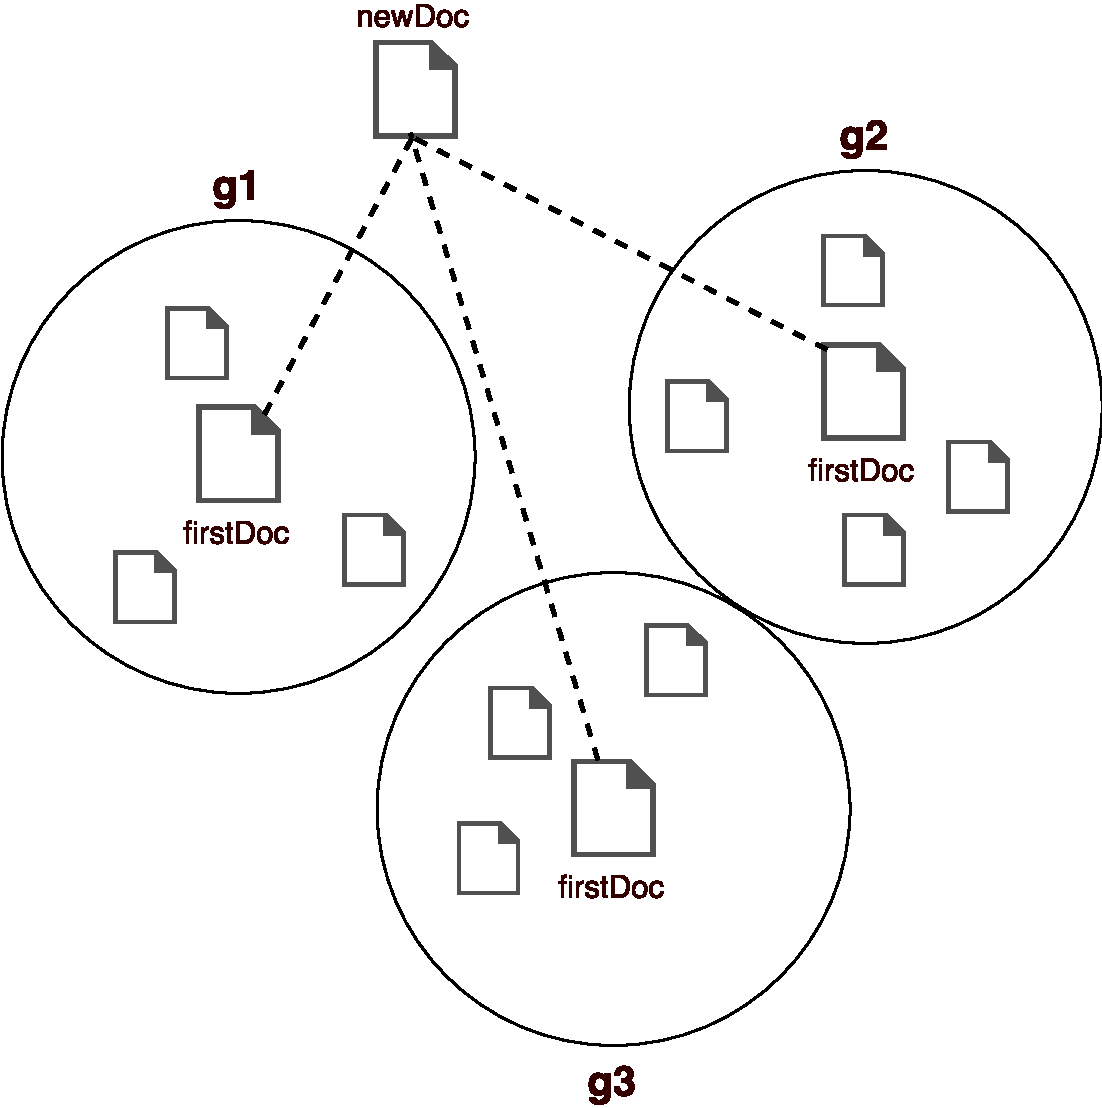
\includegraphics[width=0.65\textwidth]{Clustering_NER2.pdf}
			\caption{Cách xử lý một document mới theo thuật toán Boost Named Entity}
		\end{center}
	\end{figure}
	
	\subsubsection{Mã giả}
	\begin{algorithm}[H]
		\caption{Phát hiện tin nóng sử dụng gom cụm theo nội dung, boost Named Entity}
		\begin{algorithmic}[1]
			\REQUIRE luồng bài viết từ Twitter, giá trị ngưỡng MergeThreshold
			\ENSURE các cụm bài viết ứng với mỗi story phát hiện được, có thứ tự xếp hạng giữa các cụm

			\ForEach{document $d$ trong toàn bộ dữ liệu}
				\State $MaxScore_d \leftarrow 0$
				\State $IDMaxScore_d \leftarrow \emptyset$
				\ForEach{cụm g trong tập hợp cụm G}
%					\State tính $Score_d[g]$: độ tương đồng giữa $d$ với $g.firstDoc$, chỉ dùng một số topTerms của $g$
					\State tính $Score_d[g] \leftarrow similarity(d, g.firstDoc)$
					
					\IF{$MaxScore_d < Score_d[g]$}
						\State $MaxScore_d \leftarrow Score_d[g]$
						\State $IDMaxScore_d \leftarrow g.groupID$
					\ENDIF
				\ENDFOR
				
				\IF{$MaxScore_d$ > MergeThreshold}
					\State gán $d$ vào cụm $IDMaxScore_d$
				\ELSE
					\State tạo cụm $g_{new}$
					\State $g_{new}.firstDoc \leftarrow d$
				\ENDIF
			\ENDFOR
		\end{algorithmic}
	\end{algorithm}
	Chú thích thuật toán:
	\begin{itemize}
		\item $MaxScore_d$: chứa độ tương đồng lớn nhất giữa document d và các cụm đã có
		\item $IDMaxScore_d$: ID của cụm tương đồng nhất với document d
		\item $Score_d[g]$: độ tương đồng giữa document d với cụm g 
		\item $MergeThreshold$: ngưỡng để xét một document có thuộc về cụm/có là first story hay không
	\end{itemize}
	Độ tương đồng giữa 2 document được tính bằng các công thức sau:
	\begin{equation}
			similarity(d_1, d_2) = \sum_{t \in d_1,\ t \in g.topTerms}[tf(t, d_2) \times idf(t) \times boost(t)]
	\end{equation}
	\begin{equation}
		tf(t, d) = \frac{count(t \in d)}{size(d)}
	\end{equation}
	\begin{equation}
		idf(t) = 1 + \log\frac{N}{count(m\ has\ t)}
	\end{equation}
	Các kí hiệu: 
	\begin{itemize}
		\item $similarity(d_1, d_2)$: độ tương đồng giữa document $d_1$ và document $d_2$
		\item $boost(t)$: giá trị boost cho term t, nếu t là một danh từ riêng (Named Entity) thì boost(t) > 1, ngược lại boost(t) = 1
		\item $tf(t, d)$: tần suất xuất hiện (theo phần trăm) của term t trong document d
		\item $count(t \in d)$: tần suất term t xuất hiện trong trong document d
		\item $size(d)$: số lượng term của document d
		\item $idf(t)$: giá trị inverse document frequency của term t
		\item $N$: tổng số document trong hệ thống
		\item $count(m\ has\ t)$: số document có chứa term t
	\end{itemize}

	\subsubsection{Ưu điểm, hạn chế}
	Ưu điểm:
	\begin{itemize}
		\item Dễ gom nhóm được các sự kiện bàn về cùng thực thể nào đó.
	\end{itemize}
	Nhược điểm:
	\begin{itemize}
		\item Chất lượng kết quả gom cụm phụ thuộc một phần vào việc phát hiện được thực thể có tên.
	\end{itemize}

%========================================================================================================================
\subsection{Thuật toán Locality Sensitive Hashing}
	\subsubsection{Ý tưởng}
%	(O(nd) với n là số lượng document hiện có và d là số chiều của mỗi document)
	Thuật toán tìm kiếm láng giềng gần nhất tốn rất nhiều chi phí khi lượng dữ càng lớn. Thay vào đó, ta có thể giải bài toán tìm \textit{xấp xỉ} láng giềng gần nhất. Một thuật toán để giải quyết bài toán này là \textit{Locality Sensitive Hashing (LSH)} được đề xuất bởi Piotr Indyk và cộng sự \cite{Indyk:LSH-Definition}.
	
	LSH hoạt động bằng cách chia không gian biểu diễn dữ liệu thành nhiều vùng riêng biệt bằng một tập các siêu phẳng ngẫu nhiên. Ta có thể xem mỗi cách chia không gian này ứng với một hash table, và số bit của hash code bằng với số lượng siêu phẳng đã dùng để chia không gian. Mỗi khi một document mới vào hệ thống, ta tính hash code của nó. Khi cần tìm láng giềng cho một document, ta chỉ cần so sánh nó với các document thuộc chung vùng không gian (ứng với một bucket trong hash table), nhờ đó giảm đáng kể chi phí tính toán.
	
%	Ta có thể thấy khi tăng số lượng siêu phẳng lên thì số lượng document rơi vào cùng một vùng không gian sẽ càng giảm, do kích cỡ của vùng không gian nhỏ, th
	
	Vì các siêu phẳng được chọn một cách ngẫu nhiên, nên đôi khi các document dù gần nhau vẫn có thể bị phân vào vùng khác nhau. Do đó ta thường dùng cùng lúc nhiều hash table để tăng thêm khả năng tìm được láng giềng gần nhất.	
%	LSH sử dụng một họ hash function (hàm băm) có đặc điểm: những documents càng tương đồng với nhau thì càng có khả năng trùng hash code (mã băm) với nhau. Mỗi document mới sẽ được đưa qua hash function tính toán, và sau đó được so sánh với các document có cùng hash code với nó.\\

	\subsubsection{Minh họa cách tính hash code cho LSH}
%	Xét trường hợp một document $d$ biểu diễn dưới dạng vector $d = (0,1,0,1,1,1,0)$, và ta chọn sử dụng hash code có 4 bit (dùng 4 siêu phẳng để chia không gian dữ liệu).\\
%	Mỗi hash table được khởi tạo bằng cách: tạo 4 vector ngẫu nhiên ứng với 4 siêu phẳng, số chiều bằng với số chiều vector $d$
%	Cách tính hash code của document $d$ trong một hash table như sau: lần lượt tính tích vô hướng của vector $d$ với từng vector của siêu phẳng, nếu tích dương thì bit đó có giá trị 1, nếu tích âm thì có giá trị 0. 
		
	Giả sử ta có không gian biểu diễn document gồm 7 từ/term khác nhau (8 chiều). Xét một document $d$ biểu diễn dưới dạng vector $d = (0,1,0,1,1,1,0)$, và ta chọn sử dụng hash code có 4 bit (dùng 4 siêu phẳng để chia không gian dữ liệu).
	
	Mỗi hash table được khởi tạo bằng cách: tạo 4 vector ngẫu nhiên ứng với 4 siêu phẳng, số chiều bằng 7, ứng với số chiều của vector $d$.
	
	Cách tính hash code của document $d$ trong một hash table như sau: lần lượt tính tích vô hướng của vector $d$ với từng vector của các siêu phẳng, nếu tích dương thì bit đó có giá trị 1, nếu tích âm thì có giá trị 0. 
	
	\begin{figure}[ht]
		\begin{center}
			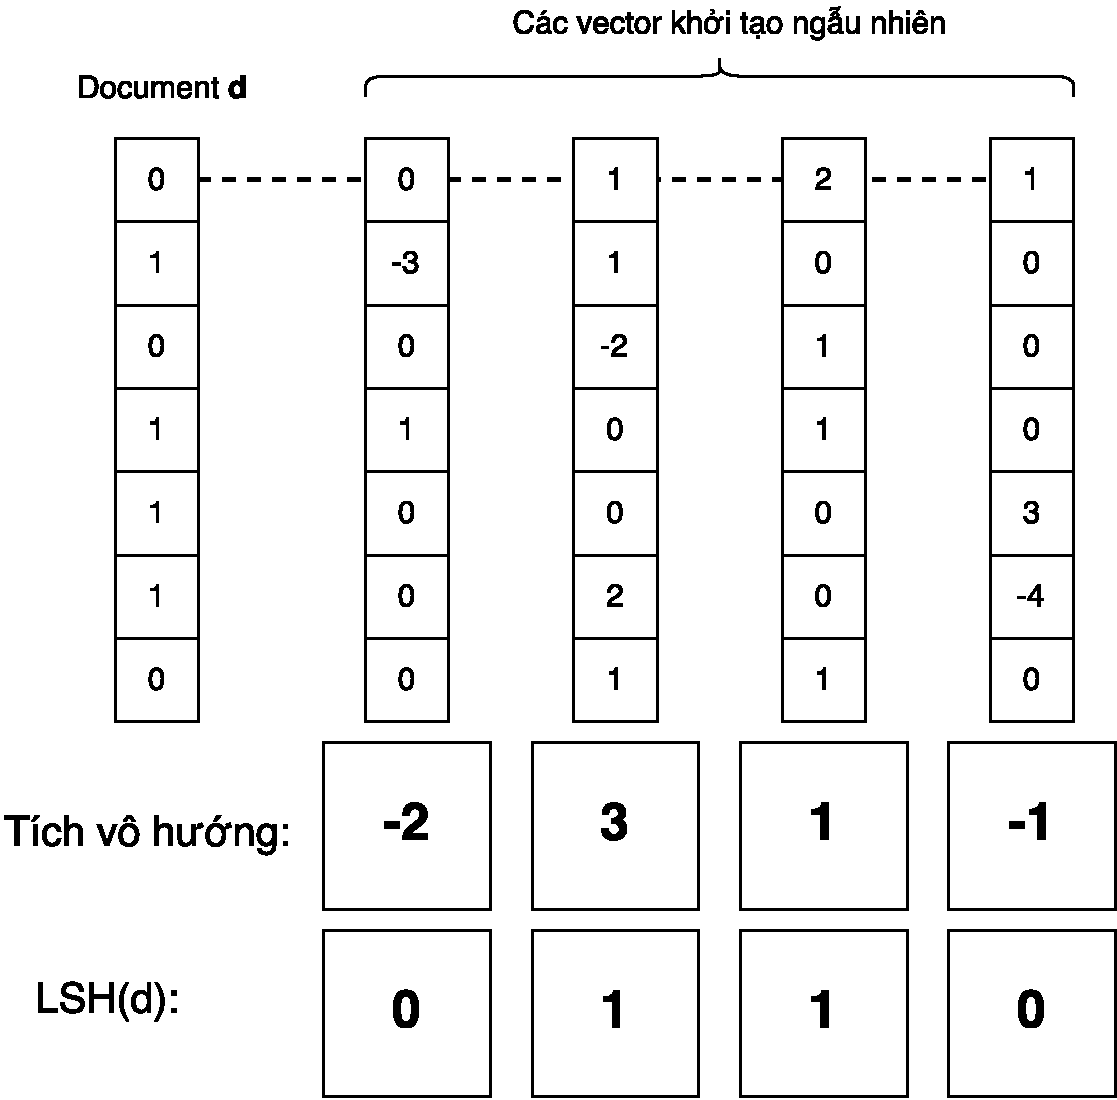
\includegraphics[width=0.65\textwidth]{LSH.pdf}
			\caption{Cách tính hash code cho một document trong một hash table}
		\end{center}
	\end{figure}
	
	\subsubsection{Mã giả}
	\begin{algorithm}[H]
		\caption{Phát hiện tin nóng sử dụng Locality Sensitive Hashing}
		\begin{algorithmic}[1]
			\REQUIRE luồng bài viết từ Twitter, giá trị ngưỡng t
			\ENSURE những cụm bài viết
			\State Khởi tạo L hash tables
			\ForEach{document $d$ mới}
				\ForEach{hash table $l$ trong $L$}
					\State Tính hash code cho document d: $LSH_l(d)$
					\State Thêm tất cả các documents d' có $LSH_l(d') = LSH_l(d)$ vào tập $S$
				\ENDFOR
				\State $dis_{min}(d) = 1$
				\ForEach{document $d'$ trong $S$}
					\IF {$distance(d,d') < dis_{min}(d)$}
					\STATE $dis_{min}(d) = distance(d,d')$
		 			\ENDIF
				\ENDFOR
				\IF{$dis_{min}(d) >= t$}
					\STATE tạo cụm mới chứa d
				\ELSE
					\STATE thêm d vào cụm chứa hàng xóm gần nhất của d
				\ENDIF
			\ENDFOR
			
		\end{algorithmic}
	\end{algorithm}
	Chú thích thuật toán:
	\begin{itemize}
		\item $t$: ngưỡng để xét một document có phải là first story hay không
		\item $LSH_l(d)$: hash code của document $d$ trong hash table thứ $l$
		\item $dis_{min}(d)$: khoảng cách giữa document $d$ với document gần nhất
		
	\end{itemize}
	
	Ưu điểm:
	\begin{itemize}
		\item Chi phí tính toán thấp do không cần so sánh toàn bộ các document với nhau.
		\item Độ chính xác tương đối tốt
	\end{itemize}

	Nhược điểm:
	\begin{itemize}
		\item Cần tìm chọn các thông số như: số lượng hash table, số lượng bit trong hash code,... tốt để cho kết quả chính xác.
		\item Có thể không tìm được document thật sự tương đồng nhất, trong trường hợp các điểm không được chia vào cùng vùng trong không gian do cách thiết lập của các siêu phẳng trong hash tables.
	\end{itemize}
	
	\subsubsection{LSH cải tiến}
	Dựa vào dữ liệu thực nghiệm của mình, Sasa Petrovic và cộng sự \cite{Petrovic:LSH} đưa ra nhận định rằng việc áp dụng LSH thuần túy vào bài toán FSD cho ra kết quả chưa tốt. Trong trường hợp điểm dữ liệu cách xa tất cả điểm còn lại, LSH không tìm được láng giềng gần nhất, do không có điểm nào khác rơi vào cùng bucket trong các hash table, dẫn đến không có điểm dữ liệu khác để so sánh. 
	
	Để giải quyết vấn đề này, Petrovic đưa ra phương án: mỗi khi tìm ra document $d$ có $dis_{min}(d)$ lớn hơn ngưỡng, ta áp dụng thuật toán tìm láng giềng gần nhất giữa document $d$ và khoảng 1000 tới 3000 document có thời gian gần đây nhất trong hệ thống, cập nhật giá trị $dis_{min}(d)$ và xét xem nó vẫn vượt ngưỡng hay không, nếu có thì ta kết luận $d$ là một first story, ngược lại ta cho $d$ vào cụm của láng giềng gần nó nhất.
	
	\begin{algorithm}[H]
		\caption{Phát hiện tin nóng sử dụng Locality Sensitive Hashing kết hợp với Nearest Neighbor Search}
		\begin{algorithmic}[1]
%			\boldmath
			\REQUIRE luồng bài viết từ Twitter, giá trị ngưỡng t
			\ENSURE những cum bài viết
			\State Khởi tạo L hash tables
			\ForEach{document $d$ mới}
				\ForEach{hash table $l$ trong $L$}
					\State Tính hash code cho document d: $LSH_l(d)$
					\State Thêm tất cả các documents d' có $LSH_l(d') = LSH_l(d)$ vào tập $S$
				\ENDFOR
				\State $dis_{min}(d) = 1$
				\ForEach{document $d'$ trong $S$}
					\unboldmath
					\IF {$distance(d,d') < dis_{min}(d)$}
					\State $dis_{min}(d) = distance(d,d')$
					\ENDIF
				\ENDFOR
				\IF{$dis_{min}(d) >= t$}
					\State Tính khoảng cách giữa d với một lượng (1000-3000) documents mới nhất trong bộ dữ liệu, cập nhật $dis_{min}(d)$ nếu có thay đổi.
				\ENDIF
				\IF{$dis_{min}(d) >= t$}
					\STATE tạo cụm mới chứa d
				\ELSE
					\STATE thêm d vào cụm chứa hàng xóm gần nhất của d
				\ENDIF
			\ENDFOR		
			
		\end{algorithmic}
	\end{algorithm}

\section{Giới thiệu một số độ đo đánh giá phân lớp} \label{clusterEvalMetrics}
Đánh giá chất lượng của kết quả gom cụm là nhiệm vụ khó khăn và phức tạp, do bản chất không hoàn toàn rõ ràng về định nghĩa của một "cụm". Theo tác giả Pang-Ning Tan và cộng sự \cite{IntroToDM}, có 3 loại phương pháp để đánh giá chất lượng cụm: 
	\begin{itemize}
		\item Đánh giá ngoại, có giám sát (External evaluation): Các độ đo có sử dụng thông tin bên ngoài như nhãn lớp của dữ liệu để so sánh với kết quả gom cụm.
		VD: Purity, Rand measure,...
		\item Đánh giá nội, không giám sát (Internal evaluation): Chỉ dựa vào các thông tin, thuộc tính có sẵn trong cụm để đánh giá.
		VD: Silhouette index, Dunn index, Davies–Bouldin index...
		\item Đánh giá tương đối (Relative evaluation): So sánh kết quả giữa các phương pháp gom cụm hoặc giữa các cụm, có thể dùng độ đo ngoại lẫn nội.
	\end{itemize}

%Khóa luận này chỉ xem xét đến các chỉ số đánh giá nội, do hạn chế về mặt dữ liệu tin tức có gán nhãn lớp.
	\subsection{Khoảng cách cục bộ và toàn cục (Intra-cluster và Inter-cluster distance)} \label{localglobaldistance}
	Hai độ đo này thuộc loại đánh giá nội, chỉ dựa vào chính dữ liệu được gom cụm để tính giá trị của chúng. Khoảng cách cục bộ của một cụm thể hiện mức độ các điểm dữ liệu trong một cụm tương đồng với nhau thế nào. Dưới đây là 3 cách để tính khoảng cách cục bộ:
		\begin{itemize}
			\item Dùng khoảng cách giữa 2 điểm xa nhau nhất trong cụm:\\
			\scalebox{1.1}{$intraclusterDistance(C_i) = \ max_{x, y \in C_i} distance(x, y)$}
			
			\item Dùng trung bình khoảng cách giữa tất cả cặp điểm trong cụm:\\
			\scalebox{1.1}{$intraclusterDistance(C_i) = \frac{1}{size(C_i) \ *\ [size(C_i)-1]} \sum_{x, y \in C_i, x \ne y} distance(x, y)$ }\\
			
			\item Dùng trung bình khoảng cách giữa từng điểm với tâm cụm:\\
			\scalebox{1.1}{$intraclusterDistance(C_i) = \frac{\sum_{x \in C_i} distance(x, \mu)}{size(C_i)} $, $\mu = \frac{\sum_{x \in C_i} x}{size(C_i)}$}\\	
		\end{itemize}
	
	Khoảng cách toàn cục là giá trị cho thấy mức độ rời rạc giữa tất cả các cụm với nhau, được tính bằng trung bình khoảng cách giữa các cụm:
		\begin{equation}
			interclusterDistance = \frac{1}{size(C) * [size(C)-1]} \sum_{C_i, C_j \in C} distance(C_i, C_j)
		\end{equation}
	
	Trong đó, khoảng cách giữa 2 cụm $distance(C_i, C_j)$ cũng có thế được xác định bằng nhiều cách như:
		\begin{itemize}
			\item Dùng khoảng cách giữa 2 điểm xa nhau nhất trong 2 cụm:\\
			\scalebox{1.1}{$distance(C_i, C_j) = \ max_{x \in C_i, y \in C_j} distance(x, y)$}
			
			\item Dùng trung bình khoảng cách giữa tất cả cặp điểm trong 2 cụm:\\
			\scalebox{1.1}{$distance(C_i, C_j) = \frac{1}{size(C_i) + size(C_j)} \sum_{x \in C_i, y \in C_j} distance(x, y)$ }
			
			\item Dùng khoảng cách giữa 2 tâm cụm:\\
			\scalebox{1.1}{$distance(C_i, C_j) = distance(\mu_{C_i}, \mu_{C_j})$, với $\mu_{C_i} = \frac{\sum_{x \in C_i} x}{size(C_i)}$}
%			\scalebox{1.1}{$\mu_{C_i} = \frac{\sum_{x \in C_i} distance(x, \mu)}{size(C_i)}$}\\	
	\end{itemize}

	Chú thích kí hiệu: 
	\begin{itemize}
		\item $C_i$: cụm dữ liệu thứ $i$
%		\item $localDistance(C_i)$: khoảng cách cục bộ của cụm $i$
		\item $x, y$: 2 điểm dữ liệu bất kì
		\item $distance(x, y)$: khoảng cách giữa 2 điểm dữ liệu, dùng các khoảng cách ở mục \ref{distances}
		\item $size(C_i)$: số lượng điểm dữ liệu được gom vào cụm $i$
	\end{itemize}
	\subsection{Độ đo Dunn index}
	Dunn index được đề xuất bởi J. C. Dunn \cite{dunn1973fuzzy2}, độ đo này thể hiện mức độ gắn kết của từng cụm lẫn độ rời rạc giữa các cụm. Giá trị Dunn index được tính theo công thức sau:	
		\begin{equation} \label{dunnindex}
		DI = \frac{min_{1 \leq i \leq j \leq n}distance(C_i, C_j)}{max_{1 \leq k \leq n}intraclusterDistance(k)}
		\end{equation}
		
		Với $n$ là tổng số cụm thu được, và intraclusterDistance được tính theo một trong những cách ở mục \ref{localglobaldistance}.
		
	Giá trị Dunn index càng cao thì các cụm càng tách biệt nhau và mỗi cụm thì có những điểm dữ liệu gom sát với nhau. Tuy vậy, mẫu số trong công thức (\ref{dunnindex}) lấy khoảng cách cục bộ của cụm rời rạc nhất chứ không lấy trung bình tất cả cụm, nên giá trị Dunn index là trường hợp xấu nhất chứ không phải trường hợp trung bình.
	\subsection{Hệ số Silhouette (Silhouette coefficient)}
%	Cohesion và separation
	
	Silhouette là một độ đo xem xét các đối tượng trong dữ liệu có được gán vào cụm hợp lý hay không, thông qua việc so sánh cả độ gắn kết của từng cụm và độ rời rạc giữa các cụm. Với mỗi điểm dữ liệu, giá trị silhouette coefficient nằm trong khoảng từ -1 đến 1, giá trị này cao khi điểm dữ liệu tương đồng với cụm của nó và ít tương đồng với cụm khác, và ngược lại. 
	
	Cách tính hệ số Silhouette cho một điểm dữ liệu \textbf{i} như sau:
	\begin{enumerate}
		\item Tính khoảng cách trung bình giữa i với các điểm trong cùng cụm với i. Gọi giá trị này là $a_i$.
		\item Với mỗi cụm g không chứa i, tính khoảng cách của i đến cụm g bằng trung bình khoảng cách giữa i với từng điểm trong cụm g, chọn cụm có khoảng cách đến i \textit{nhỏ nhất}. Gọi giá trị này là $b_i$
		\item Tính hệ số Silhouette theo công thức sau:
		\begin{equation}
		s(i) = \frac{b_i - a_i}{max\{a_i,b_i\}}
		\end{equation}
	\end{enumerate}
	
	Ở đây $a_i$ đại diện cho độ bất phù hợp của điểm i với cụm của nó, và $b_i$ đại diện cho độ tương đồng giữa điểm i với cụm gần nhất không chứa i. Vì vậy khi $a_i$ nhỏ, $b_i$ lớn, giá trị hệ số silhouette tiến tới 1, nghĩa là điểm dữ liệu i rất phù hợp với cụm của nó và không phù hợp với cụm khác. Trong trường hợp ngược lại, giá trị silhouette tiến tới -1.
	
	Giá trị hệ số Silhouette cho một kết quả phân cụm được tính bằng trung bình hệ số Silhouette của tất cả điểm dữ liệu.

	\subsection{Độ đo Purity}
	Đây là một độ đo đánh giá ngoại. Dựa trên nhãn lớp của dữ liệu, purity là độ đo về tính thuần khiết/độ đồng nhất của các cụm. Giá trị này tính bằng cách lấy tần số của lớp chiếm số lượng nhiều nhất trong cụm (tính theo phần trăm kích cỡ cụm). Purity càng cao khi cụm chứa càng nhiều điểm dữ liệu thuộc cùng một nhãn lớp.\\
	
	Giá trị purity của một cụm $C_i$ được tính bằng công thức:
	\begin{equation}
	purity(C_i) = max_j( \frac{m_{ij}}{m_i})
	\end{equation}
	
	Trong đó:
	\begin{itemize}
		\item $m_i$: số điểm dữ liệu thuộc cụm i
		\item $m_{ij}$: số điểm dữ liệu thuộc lớp j và nằm trong cụm i
	\end{itemize}
	
	Giá trị purity của tất cả cụm được tính như sau:
	\begin{equation}
	purity = \sum_{i=1}^{K} \frac{m_i}{m} \ purity(C_i)
	\end{equation}
	
	Trong đó:
	\begin{itemize}
		\item $K$: tổng số cụm
		\item $m$: tổng số điểm dữ liệu
	\end{itemize}
	
\section{Xếp hạng cụm}
	Một yêu cầu của bài toán phát hiện tin nóng là các chuỗi tin (ứng với các cụm) phải được sắp xếp theo mức độ nóng giảm dần. Hầu hết các phương pháp đã khảo sát trong khóa luận này chỉ tập trung vào việc gom cụm và cải thiện chất lượng cụm, mà không đề cập đến việc sắp xếp cụm theo thứ tự nào đó. 
	
	Tác giả Phuvipadawat đưa ra một số công thức để tính điểm lượng giá độ nóng của chuỗi tin, và các chuỗi tin được sắp xếp theo giá trị điểm giảm dần \cite{SwitPhuvipadawat}.
	
%	Các cụm được xếp hạng bằng công thức được đề xuất bởi Phuvipadawat \cite{SwitPhuvipadawat}, mỗi cụm được gán một giá trị điểm, và dùng điểm đó để so sánh giữa các cụm, cụm có điểm cao nhất sẽ được sắp xếp lên đầu.
	
	Điểm này cân nhắc tầm ảnh hưởng của những người viết bài trong cụm, cũng như mức độ lan tỏa của chính các bài viết trong cụm. Giá trị điểm cũng được cập nhật thường xuyên và sẽ giảm dần theo thời gian nếu không có những bài viết mới làm tăng điểm cho nó. So với công thức của Phuvipadawat, công thức 2.12 bổ sung thêm yếu tố lượng favorite của cụm, do đây cũng là một thành phần ghi nhận phản ứng từ người dùng Twitter.
	
	Giá trị điểm xếp hạng của một cụm $C_i$ được cho bằng công thức sau:
	\begin{equation}
		Score(C_i) = \frac{1}{Z} \sum_{j = 1}^k \frac{S_i}{log_2(\Delta_j + 2)}
	\end{equation}
	
	Với $S_i$ tính bằng:
	\begin{multline}
	S_i = w_1 \sum_{u_i \in C_i} FollowerCount(u_i) + w_2\ TotalRetweetCount(C_i)\\ + w_3\ TotalFavoriteCount(C_i)
	\end{multline}

	Trong đó:
	\begin{itemize}
		\item $\frac{1}{Z}$: giá trị để chuẩn hóa điểm cụm, Z là tổng điểm của các cụm khi chưa chuẩn hóa
		\item $k$: số lượng document trong cụm
		\item $\Delta_j$: chênh lệch thời gian giữa thời điểm hiện tại với thời gian bài viết $j$ được đăng
		\item $w_1, w_2$: trọng số cho hai vế của biểu thức
		\item $u_i$: người dùng thứ $i$
		\item $FollowerCount(u_i)$: số người follow người dùng $u_i$ trên Twitter
		\item $TotalRetweetCount(g_i)$: tổng số retweet của các bài đăng trong cụm $c_i$
	\end{itemize}
\section{Kết chương}
Chương này đã phát biểu bài toán phát hiện tin nóng và đưa ra 4 thuật toán tiếp cận theo hướng gom cụm. Đồng thời trình bày về các độ đo tương đồng, độ đo đánh giá chất lượng cụm và cách xếp hạng cụm. Chương tiếp theo sẽ trình bày về việc xây dựng hệ thống phát hiện tin nóng.
\renewcommand\thefigure{3.\arabic{figure}} 
\setcounter{figure}{0}
\chapter{HIỆN THỰC HỆ THỐNG LỌC RÁC TIN TỨC}
\ifpdf
    \graphicspath{{Chapter3/Chapter3Figs/PNG/}{Chapter3/Chapter3Figs/PDF/}{Chapter3/Chapter3Figs/}}
\else
    \graphicspath{{Chapter3/Chapter3Figs/EPS/}{Chapter3/Chapter3Figs/}}
\fi

\section{Mở đầu}
Chương này sẽ trình bày về thiết kế, chi tiết cài đặt, các thư viện và framework được sử dụng để xây dựng hệ thống lọc rác tin tức.

\section{Mô hình hệ thống}
Dưới đây là mô hình của các thành phần chính hệ thống:
\begin{figure}[H]
	\centering
	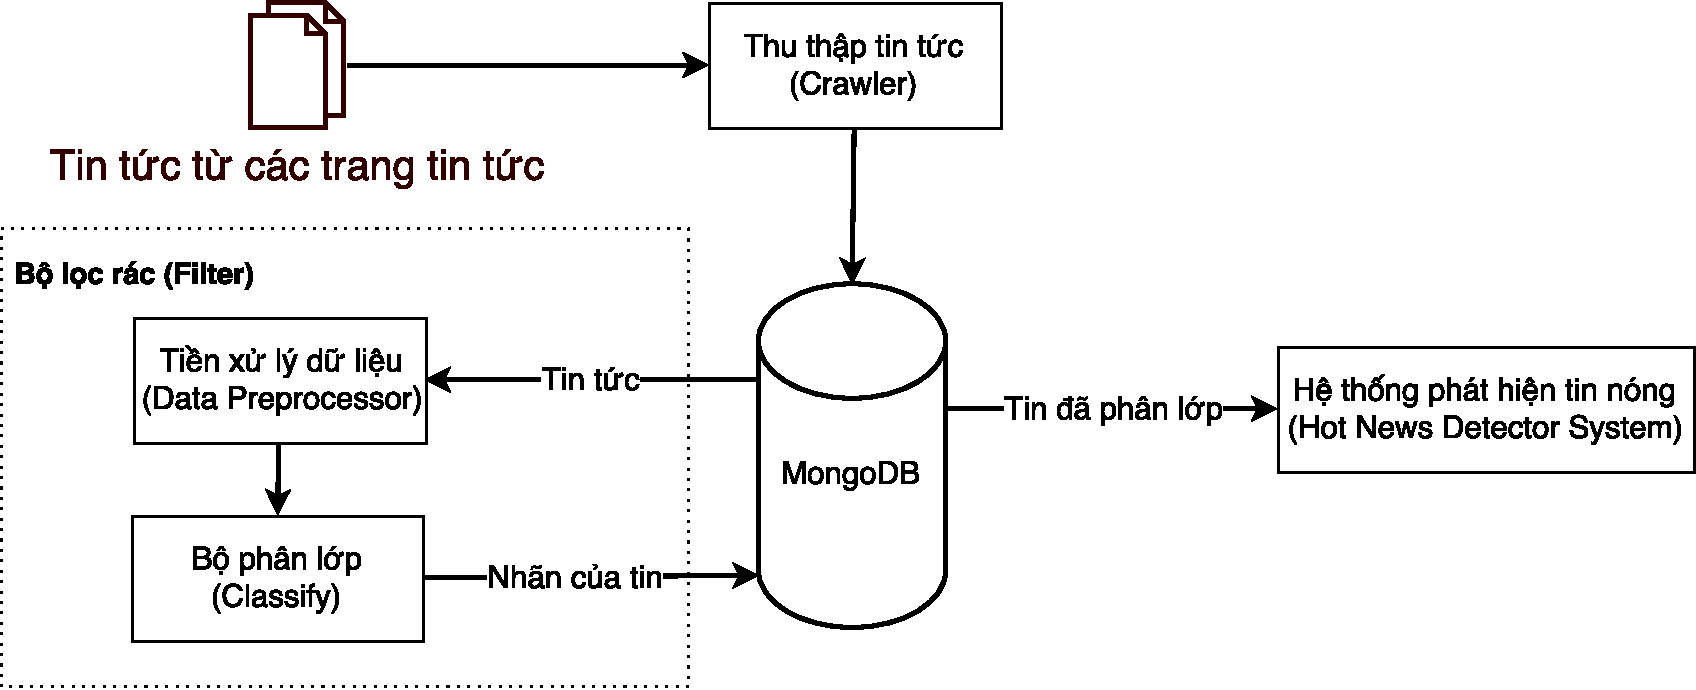
\includegraphics[width=0.9\linewidth]{Chapter3/Chapter3Figs/PDF/SystemArchitecture}
	\caption{Các thành phần chính của hệ thống}
	\label{fig:systemarchitecture}
\end{figure}
\subsection{Luồng xử lý dữ liệu}
	Hệ thống phân loại tin tức được chia thành 2 hệ thống nhỏ hơn, đó là hệ thống Crawler và hệ thống Spam Filtering: 
	\begin{itemize}
		\item Hệ thống Crawler có nhiệm vụ đồng bộ hóa tin tức đã được lấy về từ các trang tin tức và thực hiện tiến trình phân lớp(classification process) cho các tin tức đó.
		\item Hệ thống Spam Filtering cung cấp các API: phân loại tin tức bằng tiêu đề hoặc bằng URL của tin đó, cung cấp dữ liệu thống kê cho các tin đã phân lớp ở hệ thống Crawler, API feedback khi các tin dự đoán sai mong muốn của bình luận viên.
	\end{itemize}
Hệ thống Crawler phục vụ cho bài toán Hot News Detection, sau khi tin tức được lọc rác, các tin tức được đánh giá là rác sẽ bị bỏ qua khi đưa vào hệ thống Hot News Detection.
Hệ thống Spam Filtering chủ yếu phục vụ cho biên tập viên. Biên tập viên sử dụng hệ thống thông qua giao diện Spam Filtering để sử dụng chức năng phân lớp tin tức hoặc xem các số liệu thống kê về tin tức đã phân lớp lưu trong cơ sở dữ liệu.
\section{Tiến trình phân lớp}
\begin{figure}[H]
	\centering
	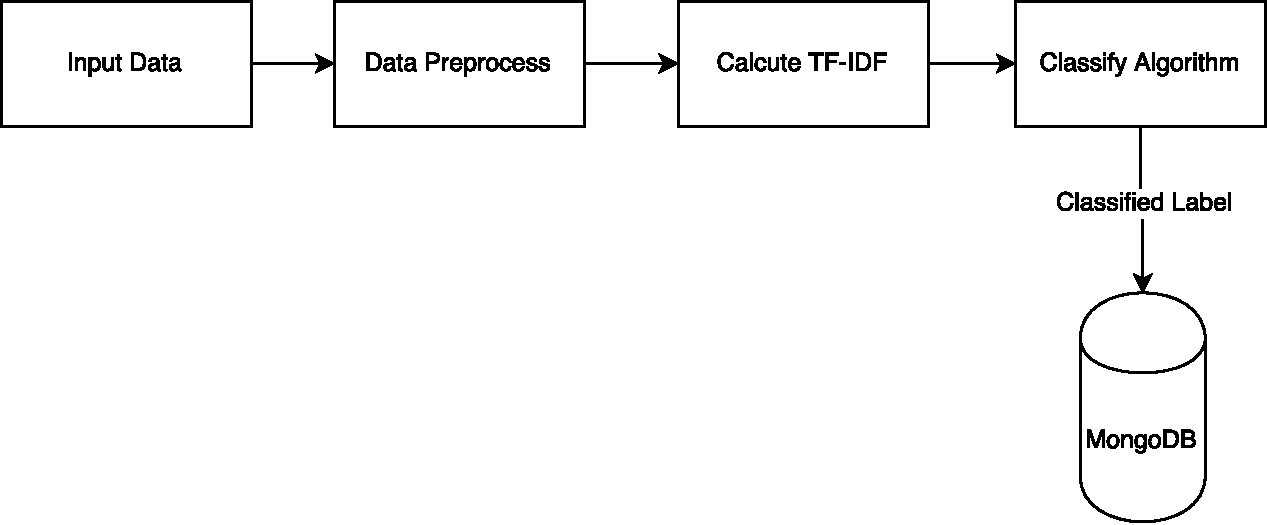
\includegraphics[width=0.9\linewidth]{Chapter3/Chapter3Figs/PDF/ClassifyProcess}
	\caption{Tiến trình phân lớp}
	\label{fig:classifyprocess}
\end{figure}
Tiến trình phân lớp sẽ bao gồm \nameref{sec:DataPreprocessor} và phân hệ Classify.
Phân hệ Classify bao gồm: \nameref{sec:newsClassify} và \nameref{sec:spamCategory}.
Luồng xử lý của tiến trình phân lớp sẽ thực thi theo hình \ref{fig:classifyprocess} :
\begin{itemize}
	\item Input data: Dữ liệu đầu vào, gồm các document bao gồm Id và title của tin được lưu dưới định dạng csv. Mỗi dòng trong file csv bao gồm 2 cột: Id và title của tin tức đó.
	\item Data Preprocess: Dữ liệu ở cột title  sẽ thực thi theo \nameref{sec:DataPreprocessor}. Output của quá trình này là file csv với cột title đã được xử lý.
	\item Calculate TF-IDF: Dữ liệu title sau khi được tiền xử lý sẽ được tính TF-IDF. Output của quá trình tính tf-idf sẽ là file csv chứa các kết quả tf-idf theo attribute của tập từ điển.
	\item Classify Algorithm: Hệ thống sẽ sử dụng thư viện Weka để phân lớp dữ liệu. Output của quá trình này sẽ là nhãn(Label) của tin. Sau đó, nhãn sẽ được lưu xuống cơ sở dữ liệu MongoDB.
\end{itemize}

\section{Phân hệ thu thập dữ liệu (Data Streaming)} \label{sec:DataStreaming}
Module này sử dụng hệ thống Crawler để lấy các bài đăng từ nhiều nguồn tin tức lưu trữ ở cơ sở dữ liệu MySQL và đưa qua cơ sở dữ liệu MongoDB, hệ thống sẽ thực hiện các chức năng:
	\begin{itemize}
		\item Connect vào cơ sở dữ liệu mySQL để lấy các bài bài báo.
		\item Xóa các bài viết trùng.
		\item Lưu trữ xuống cơ sở dữ liệu MongoDB
	\end{itemize}
\section{Phân hệ tiền xử lý dữ liệu (Data Preprocessor)}
\label{sec:DataPreprocessor}
Module tiền xử lý có nhiệm vụ chính gồm loại bỏ URL, thực hiện tách từ, loại bỏ stopwords và biểu diễn dữ liệu thành vector trọng số tf-idf. Trước khi chạy thuật toán phân loại, dữ liệu được lấy ra từ MongoDB và tiền xử lý phần nội dung của bài báo bằng các bước sau:
	\begin{enumerate}
		\item Loại bỏ URL bằng regular expression.
		\item Tách từ sử dụng thư viện TPSegmenter. Bước này dùng để biểu diễn các từ ghép trong tiếng Việt bằng cách thêm gạch nối giữa các tiếng của từ.\\
		Ví dụ: \textit{"Vụ tai nạn 13 người chết: Đã giám định mẫu máu tài xế xe tải"} qua bộ tách từ sẽ thành \textit{"Vụ tai\_nạn 13 người chết : Đã giám\_định mẫu máu tài\_xế xe\_tải"}.
		\item Loại bỏ các từ trong danh sách gồm 813 stopwords.
		\item Tính và biểu diễn dữ liệu thành vector tf-idf và metadata.
	\end{enumerate}

\section{Phân hệ phân loại tin tức}
\label{sec:newsClassify}
Sử dụng model đã train trước đó để phân loại tin tức. Model sử dụng thuật toán SVM đã trình bày ở chương 2 làm thuật toán chính để phân loại tin tức. Hiện tại hệ thống có 2 nhãn đã được định nghĩa trước đó:
	\begin{itemize}
		\item \textit Không rác
		\item \textit Rác
	\end{itemize}

Sau khi đã phân loại, hệ thống sẽ lưu nhãn đã gán cho tin tức xuống cơ sở dữ liệu MongoDB.

\section{Phân hệ phân loại loại rác}
\label{sec:spamCategory}
Hệ thống sẽ lấy những tin được gán nhãn "Rác" ở bước phân loại tin tức ở trên để phân loại loại rác cho tin đó. Hiện tại có 3 loại rác đã được định nghĩa trước:
\begin{itemize}
	\item \textit Quảng cáo
	\item \textit Tuyển dụng
	\item \textit Chia sẻ
\end{itemize}

\section{Thiết kế hệ thống} 
	\begin{figure}[H]
		\centering
		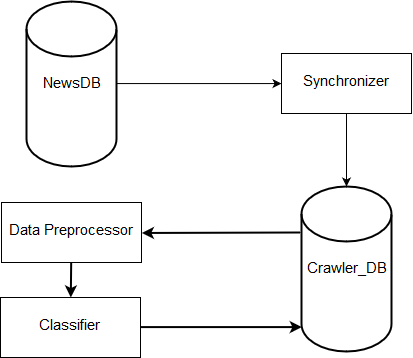
\includegraphics[width=0.5\linewidth]{Chapter3/Chapter3Figs/CrawlerSystem}
		\caption{Kiến trúc hệ thống crawler tin tức}
		\label{fig:crawlersystem}
	\end{figure}
Hệ thống Crawler được xây dựng độc lập bao gồm phân hệ thu thập dữ liệu, phân hệ tiền xử lý và phân hệ phân lớp để chạy ngầm nhằm thu thập và phân loại thông tin
	\begin{figure}[H]
		\centering
		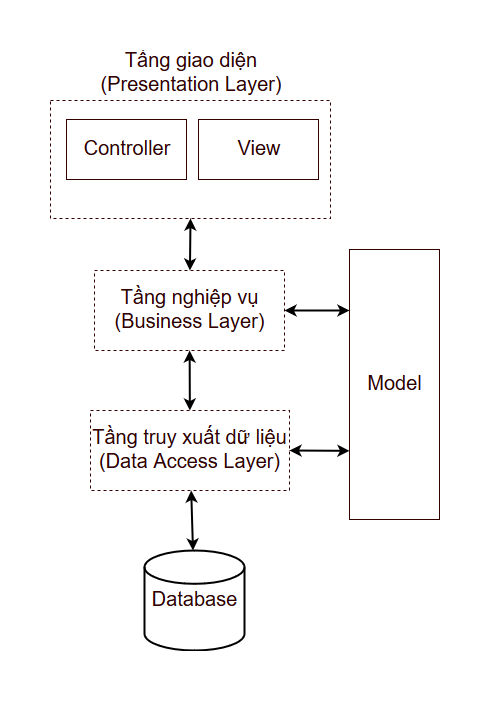
\includegraphics[width=0.5\linewidth]{Chapter3/Chapter3Figs/Layers}
		\caption{Kiến trúc hệ thống Spam Filter kết hợp Multilayer architecture kết hợp với mô hình MVC}
		\label{fig:layers}
	\end{figure}
%Hệ thống xây dựng theo kiến trúc client-server và sử dụng struts 2 framework áp dụng mô hình Model - View - Controller (MVC) với View tách biệt(sử dụng framework React) và cung cấp api để trả về kết quả dạng JSON. Cụ thể:
Hệ thống xây dựng theo kiến trúc 3 tầng gồm: Presentation Layer, Business Logic Layer và Data Access Layer. Trong đó, Presentation Layer áp dụng mô hình Model - View - Controller (MVC). Cụ thể:
	\begin{itemize}
		\item Presentation Layer: Có trách nhiệm hiển thị thông tin, tương tác với người dùng hệ thống. Gồm 2 thành phần:
			\begin{itemize}
				\item Controller: Điều khiển các luồng của hệ thống web, nhận các tín hiệu từ người dùng và xử lý tương ứng.
				\item View: Có nhiệm vụ hiển thị các giao diện hệ thống cho người dùng, hệ thống sử dụng React để gọi api trả về dữ liệu cho giao diện người dùng.
			\end{itemize}
		\item Model: Đối tượng chứa dữ liệu để xử lý và hiển thị.
		\item Business Layer: Chứa các nghiệp vụ của hệ thống. Bao gồm các bước xử lý dữ liệu, thuật toán gom cụm, các tác vụ thống kê,…
		\item Data Access Layer: Có nhiệm vụ giao tiếp với các hệ cơ sở dữ liệu.
	\end{itemize}

\section{Cài đặt hệ thống}%các packages
Hệ thống ứng dụng được xây dựng trên nền tảng Java EE với các thành phần sau:
	\begin{itemize}
		\item Ngôn ngữ: Java, HTML, CSS, JavaScript, React.
		\item Hệ cơ sở dữ liệu: MongoDB và MySQL.
		\item Thư viện, framework: Apache Struts 2, Apache Lucene, TPSegmenter, Weka
		\item Server: Apache Tomcat
	\end{itemize}

	\subsection{Các package}
	Source code chương trình được tổ chức thành các package như sau:\\
	Hệ thống crawler:
	\begin{itemize}
		\item vn.vccorp.crawler.bo: Chứa các business object của hệ thống
		\item vn.vccorp.crawler.config: Các file config cho hệ thống
		\item vn.vccorp.crawler.constant: Các file constant của hệ thống
		\item vn.vccorp.crawler.dao: Data Access Object, thực hiện các tác vụ đọc, ghi database
		\item vn.vccorp.crawler.dbconnection: Cung cấp kết nối đến database
		\item vn.vccorp.crawler.dto: Data Transfer Object, các đối tượng để vận chuyển dữ liệu từ database
		\item vn.vccorp.crawler.main: Các lớp bao đóng để tạo thread chạy song song các tác vụ
		\item vn.vccorp.crawler.thread: Các lớp bao đóng để tạo thread chạy song song các tác vụ
		\item vn.vccorp.crawler.util: Các công cụ hỗ trợ trong hệ thống
	\end{itemize}
	Hệ thống Spam Filter được tích hợp vào hệ thống HotNewsDetector:
	\begin{itemize}
		\item vn.vccorp.hotnewsdetector.action.general: lớp ảo chứa các phương thức của action.
		\item vn.vccorp.hotnewsdetector.action.news: chứa các action cho tin tức
		\item vn.vccorp.hotnewsdetector.action.twitter: chứa các action cho twitter
		\item vn.vccorp.hotnewsdetector.bo: Chứa các business object của hệ thống
		\item vn.vccorp.hotnewsdetector.config: Các file config cho hệ thống
		\item vn.vccorp.hotnewsdetector.constant: Các file constant của hệ thống
		\item vn.vccorp.hotnewsdetector.context: chứa các action context của hệ thống
		\item vn.vccorp.hotnewsdetector.crawler.news: Dùng để lấy dữ liệu từ trang web tin tức
		\item vn.vccorp.hotnewsdetector.dao: Data Access Object, thực hiện các tác vụ đọc, ghi database
		\item vn.vccorp.hotnewsdetector.dbconnection: Cung cấp kết nối đến database
		\item vn.vccorp.hotnewsdetector.dto: Data Transfer Object, các đối tượng để vận chuyển dữ liệu từ database
		\item vn.vccorp.hotnewsdetector.exception: Quản lý lỗi và đưa ra thông báo của hệ thống
		%\item vn.vccorp.hotnewsdetector.lucence: 
		%\item vn.vccorp.hotnewsdetector.luceneindex:
		\item vn.vccorp.hotnewsdetector.thread
		\item vn.vccorp.hotnewsdetector.utils
	\end{itemize}
	
	\subsection{Cơ sở dữ liệu MongoDB}
	Hệ thống sử dụng MongoDB để lưu trữ dữ liệu tin tức và quản lý kết quả phân lớp. Đây là một hệ cơ sở dữ liệu NoSQL, cung cấp khả năng mở rộng, sao lưu, phân mảnh dữ liệu tốt, và có thể thay đổi cấu trúc dữ liệu một cách linh hoạt.
	
	Dưới đây là bảng so sánh một số thuật ngữ cơ bản giữa các cơ sở dữ liệu SQL truyền thống và MongoDB:
	\begin{table}[H]
		\centering
		\setlength\extrarowheight{3pt}
		\begin{tabular}{|l|l|}
			\hline
			\textbf{Thuật ngữ SQL}	& \textbf{Thuật ngữ MongoDB}  \\\hline
			database	& database \\\hline
			table		& collection \\\hline
			row			& document hoặc BSON document \\\hline
			column		& field \\\hline
			index		& index \\\hline
			table joins	& \$lookup, embedded documents \\\hline
		\end{tabular}
		\caption{So sánh các thuật ngữ giữa SQL và MongoDB}
		\label{tab:table_3_1}
	\end{table}
	
		\subsubsection{Collection News}
		Collection này chứa thông tin về các tin lấy từ cơ sở dữ liệu MySQL, cũng là nơi lưu trữ tất cả thông tin về tweet trong hệ thống. Khi dữ liệu được stream từ MySQL về, mỗi tin chỉ có 12 trường, các trường khác sẽ được thêm vào trong quá trình hệ thống xử lý.
		\begin{table}[H]
			%				\centering
			\setlength\extrarowheight{3pt}
			\begin{tabular}{|l|l|p{7.25cm}|}
				\hline
				\textbf{Thuộc tính}     & \textbf{Loại} & \textbf{Ý nghĩa} \\\hline
				\_id           & ObjectID       & ID trong MongoDB của document \\\hline
				Id        & Int           & ID của tin tức lấy về\\\hline
				Title         & String           & Title của tin tức\\\hline
				Content & String         & Nội dung của tin tức\\\hline
				Source   & String         & Nguồn trang báo điện tử của tin tức\\\hline
				CreateTime  & Date           & Thời gian đăng của tin\\\hline
				GetTime    & Date           & Thời gian tin tức được thu thập vào cơ sở dữ liệu MySQL\\\hline
				CollectDate    & Date           & Thời gian tweet được thu thập vào cơ sở dữ liệu MongoDB\\\hline
				Author  & String        & Người viết bài báo(nếu có)\\\hline
				Category   & Integer        & Chủ đề của bài báo\\\hline
				SpamLabel & String        & Nhãn đã gán cho tin tức\\\hline
				SpamCategory   & String         & Nhãn đã gán cho loại tin rác\\\hline
				SpamLabelFeedback      & Integer        & Feedback của nhãn đã gán cho tin tức đó\\\hline
			\end{tabular}%
			
			\caption{Các trường của collection News}
			\label{tab:table_3_2}%
		\end{table}%
		
		\subsubsection{Collection HashCode}
		Collection cluster chứa các hash code cho bài báo để kiểm tra trùng cho tin tức đó.
		\begin{table}[H]
			%				\centering
			\setlength\extrarowheight{3pt}
			\begin{tabular}{|l|l|p{9cm}|}
				\hline
				\textbf{Thuộc tính}     & \textbf{Loại} & \textbf{Ý nghĩa} \\\hline
				\_id           & ObjectID       &  ID trong MongoDB của cụm\\\hline
				HashCode      & String           & Hash code của tin tức\\\hline
			\end{tabular}%
			\caption{Các trường của collection HashCode}
			\label{tab:table_3_3}%
		\end{table}%
\section{Các API hệ thống HotNewsDetector}
Hệ thống HotNewsDetector cung cấp các API:
\subsection{Classified News List}
Lấy và hiển thị các tin đã được phân loại và gán nhãn “Không rác” hoặc “Rác” trong một ngày \\
\textbf{URL:}

/HotNewsDetector/news/spam/list\\
\textbf{Request Method:}

GET\\
\textbf{Data Params:}
	\begin{itemize}
		\item startDate (String): chuỗi thể hiện ngày cần lấy tin với định dạng “dd-MM-yyyy”. Lưu ý ngày trong CSDL được lưu theo múi giờ UTC+0:00.
		\item offset (Integer, optional): số lần lượt bỏ các tin đầu tiên theo limit (số tin lượt bỏ = offset * limit). Mặc định là 0. Giá trị phải là số nguyên không âm.
		\item limit (Integer, optional): số tin tối đa cần lấy từ danh sách trả về (sau khi đã sắp xếp và lược bỏ). Giá trị phải là số nguyên không âm và nhỏ hơn 50. Giá trị mặc định là 10.
	\end{itemize}
\textbf{Success Response:}	
\lstset{
	string=[s]{"}{"},
	stringstyle=\color{blue},
	comment=[l]{:},
	commentstyle=\color{black},
	escapeinside={\%*}{*)},
	tabsize =4,
}
\begin{lstlisting}
{
	"error": false,
	"data": "[{	
		"title": "...",	
		"postdate": "...",	
		"id": "...",	
		"source": "...",	
		"SpamLabel": "...",	
		"spamCategory": "...",	
		"spamLabelFeedback": "...",	
		"url": "..."	
	},...]"
}
\end{lstlisting}
\textbf{Error Response}
\begin{lstlisting}
	"error": true,		
	"message": "..."
\end{lstlisting}
\textbf{Attributes}
	\begin{itemize}
		\item id(String): ID của tin.	
		\item title(String): tiêu đề tin.	
		\item source(String): nguồn post tin.	
		\item postDate(String): ngày đăng tin.	
		\item spamLabel(String): nhãn của tin đã được phân loại, nhãn của tin có thể có 3 giá trị: Rác, Không rác hoặc null nếu chưa phân loại.
		\item spamCategory(String): nhãn của loại rác mà tin rác được phân loại, nhãn của loại rác có thể có 4 giá trị: Quảng cáo, Tuyển dụng, Chia sẻ hoặc null nếu tin được phân loại là “Tin” hoặc chưa phân loại.
		\item spamLabelFeedback(String): phản hồi của người dùng về nhãn mà tin được tiên đoán. Có thể là “Tin”, “Rác” hoặc null.
		\item url(String): đường dẫn tới tin.
	\end{itemize}
\textbf{Sample Call}
\begin{lstlisting}
	axios.get("/HotNewsDetector/news/spam/list", {params:{startDate="11-12-2017", offset=2, limit=5}})
	.then(response => {	console.log(response);
	});
\end{lstlisting}
\subsection{Spam Label Feedback}
Cho phép người dùng phản hồi về nhãn của một tin (Rác, Tin) \\
\textbf{URL:} 

    /HotNewsDetector/news/spam/feedback \\
\textbf{Request Method:}

POST\\
\textbf{Data Params:}
\begin{itemize}
	\item spamFeedback(Integer, optional): giá trị feedback người dùng. Các giá trị có thể sử dụng: 0 (Rác), 1 (Tin).
	\item id(String): ID của tin.
\end{itemize}
\textbf{Success Response:} 
\begin{lstlisting}
{
	"error": false,
	"message": "%*Thao tác thành công*)"
}
\end{lstlisting}
\textbf{Error Response}
\begin{lstlisting}
	"error": true,		`
	"message": "..."
\end{lstlisting}
\textbf{Attributes}
\begin{itemize}
	\item error(Boolean): Kết quả trả về, true nếu có lỗi và false nếu thành công. 
	\item message(String): Thông báo thông tin cho người dùng.
\end{itemize}
\textbf{Sample Call}
\begin{lstlisting}
	axios.get("/HotNewsDetector/news/spam/list",
	{params:{startDate="11-12-2017", offset=2, limit=5}})
	.then(response => { console.log(response);
	});
\end{lstlisting}
\subsection{Spam Filter}
Cho phép người dùng phân loại một tin. Đầu vào của API có thể là danh sách chứa các URL của các tin hoặc một chuỗi String là title của các bài viết. \\
\textbf{URL:}

/HotNewsDetector/news/spam\\
\textbf{Request Method:}

POST\\
\textbf{Data Params:}
\begin{itemize}
	\item data(String[]): mảng chứa nội dung của các tin cần phân lớp, có thể là URL hoặc title của tin. Có thể nhận vào một hoặc nhiều tin cùng một lúc.
	\item type(int): xác định thuật toán sử dụng để phân lớp, có 2 giá trị có thể sử dụng: 0( Sử dụng thuật toán SVM), 1( Sử dụng Doc2Vec).
\end{itemize}
\textbf{Success Response:}
\begin{lstlisting}
{
	error: false,
	data: [{
		"label": "...",
		"type": "...",
		"content": "..."}
	},...]
}
\end{lstlisting}
\textbf{Error Response}
\begin{lstlisting}
	"error": true,		
	"message": "..."
\end{lstlisting}
\textbf{Attributes}
\begin{itemize}
	\item label(String):  nhãn của tin đã phân lớp: Tin, Rác(Quảng cáo, tuyển dụng, chia sẻ) nếu loại tin là URL, nhãn của tin có thể là Undefined nếu không lấy được tin về từ web.
	\item type(String):  loại tin đã nhập (URL hoặc Text)
	\item content (String):  Nội dung đã nhập (URL hoặc nội dung tin)
	
\end{itemize}
\textbf{Sample Call}

axios.get("{\color{blue}{/HotNewsDetector/news/spam?data}}= Trà Ngọc Hằng Thà cô đơn chứ 

không đổi tự trọng lấy tình yêu"\&type=0")

	.then(response => \{ console.log(response);
	
	\});
\subsection{Spam statistic}
Lấy các thông số thống kê về số lượng tin đã phân lớp theo khoảng thời gian và theo nguồn tin \\
\textbf{URL:} 

/HotNewsDetector/news/spam/statistics\\
\textbf{Request Method:}

GET\\
\textbf{Data Params:}

dateRange(Integer): số ngày cần lấy dữ liệu thống kê, chỉ nhận các giá trị 1, 7, 30, và 365
\textbf{Success Response:}	
\begin{lstlisting}
	"error": false,
	"data": [
	{
		"bySource": [{
		"source": ...,
		"news": ...,
		"spams": ...
	
	},...],
		"byTime": [{
		"categories": ...,
		"news": ...,
		"spam": ...
	}, ...]}
]
\end{lstlisting}
\textbf{Error Response}
\begin{lstlisting}
	"error": true,		
	"message": "..."
\end{lstlisting}
\textbf{Attributes}
\begin{itemize}
	\item (String): dữ liệu thống kê theo nguồn đưa tin.
	\item byTime(String): dữ liệu thống kê theo khoảng thời gian.
	\item source(String): tên nguồn tin.
	\item categories(String): khoảng thời gian đã phân chia, khoảng thời gian có thể có 4 giá trị tùy theo dateRange đã nhập:
	\begin{itemize}
		\item Date range = 1: khoảng thời gian sẽ được chia làm 12 phần, mỗi phần tương ứng 2 tiếng
		\item 	Date range = 7: khoảng thời gian được chia làm 7 phần, mỗi phần tương ứng 1 ngày.
		\item 	Date range = 30: khoảng thời gian được chia làm 15 phần, mỗi phần tương ứng 2 ngày.
		\item 	Date range = 365: khoảng thời gian được chia làm 12 phần, mỗi phần tương ứng 1 tháng.
	\end{itemize}
	\item news(String): số lượng tin đã phân lớp “Không rác”
	\item spam(String): số lượng tin đã phân lớp là “Rác”
\end{itemize}	
\textbf{Sample Call}
\begin{lstlisting}
	axios.get("/HotNewsDetector/news/spam/statistics", { params:{dateRange:7} })
	.then(response => { console.log(response);
	}); 

\end{lstlisting}

\section{Giao diện}
Giao diện hệ thống được xây dựng sử dụng thư viện React, với kiến trúc Redux. Giao diện tương tác với hệ thống thông qua ajax request.
	\begin{figure}[H]
		\centering
		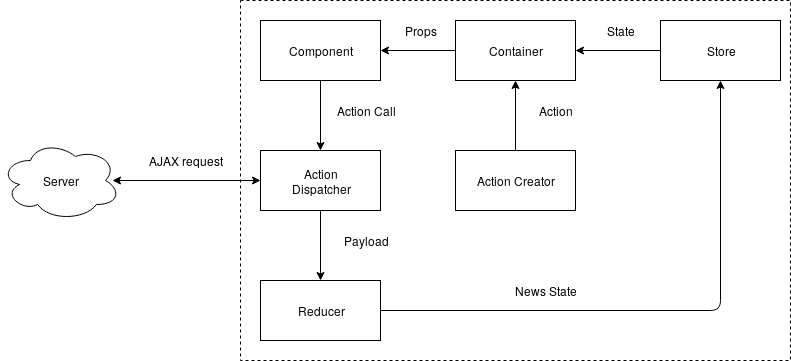
\includegraphics[width=1\linewidth]{Chapter3/Chapter3Figs/FrontEndArch}
		\caption{Kiến trúc giao diện hệ thống}
		\label{fig:layers}
	\end{figure}

  \subsection{Giao diện danh sách tin đã phân lớp}
  \begin{table}[H]
    \centering
    \setlength{\tabcolstep}{12pt}
    \begin{tabular}{@{}lll@{}} \toprule
      Tên  & Loại   & Mô tả \\ \midrule
      fetchSpam &  Action   & Truy xuất danh sách các tin đã phân lớp \\
      sendFeedback & Action & Gửi phản hồi người dùng về label của tin đã phân lớp \\
      spamList     & State       & Danh sách các tin đã phân lớp  \\ \bottomrule
    \end{tabular}
    \caption{Bảng các thuộc tính}
  \end{table}
  \begin{table}[H]
    \centering
    \setlength{\tabcolstep}{12pt}
    \begin{tabular}{@{}lll@{}} \toprule
      Tên  & Loại   & Mô tả \\ \midrule
      Date  &  Date Picker & Chọn ngày để lấy danh sách tin đã phân lớp \\
      SpamTable  & Table & Hiển thị danh sách các tin đã phân lớp \\
      FeedbackBox & Select & Chọn và gửi phản hồi về label của tin đã phân lớp \\ \bottomrule
    \end{tabular}
    \caption{Bảng các đối tượng hiển thị}
  \end{table}

  \subsection{Giao diện phân lớp tin}
  \begin{table}[H]
    \centering
    \setlength{\tabcolstep}{12pt}
    \begin{tabular}{@{}lll@{}} \toprule
      Tên  & Loại   & Mô tả \\ \midrule
      fetchLabels &  Action   &  Gửi danh sách các tin cần phân lớp và lấy về các label tương ứng \\
      spamLabels  &  State  & Danh sách các tin và label tương ứng \\ \bottomrule
    \end{tabular}
    \caption{Bảng các thuộc tính}
  \end{table}

  \begin{table}[H]
    \centering
    \setlength{\tabcolstep}{12pt}
    \begin{tabular}{@{}lll@{}} \toprule
      Tên  & Loại   & Mô tả \\ \midrule
      InputTable   &  Table & Bảng chứa các tin cần hoặc đã phân lớp \\
      DatatypeMenu   & Tabs & Chuyển kiễu dữ liệu của input: text hoặc URL \\
      ClassifyButton  & Button  & Thực hiện phân lớn các input \\
      InputButton   & Button & Hiển thị input form \\
      InputForm   & Form, Popup & Form để thêm input mới \\
      ContentText & Input & Nội dung input \\
      ExpectedLabel & Select & Label mong đợi của input \\
      ConfirmButton & Button & Thêm input mới vào table của tab hiện tại \\
      ImportButton & Button & Truyền dữ liệu input từ file \\
      ClearAllButton & Button & Xóa hết dữ liệu input từ table của tab hiện tại \\
      DeleteButton & Button & Xóa một dòng input trên bảng \\ \bottomrule
    \end{tabular}
    \caption{Bảng các đối tượng hiển thị}
  \end{table}
  \subsection{Giao diện thống kê dữ liệu phân lớp}
  \begin{table}[H]
    \centering
    \setlength{\tabcolstep}{12pt}
    \begin{tabular}{@{}lll@{}} \toprule
      Tên  & Loại   & Mô tả \\ \midrule
      fetchSpamStatistics &  Action   &  Truy xuất dữ liệu thống kê phân lớp \\
      spamStatistics  &  State  & Dữ liệu thống kê phân lớp \\ \bottomrule
    \end{tabular}
    \caption{Bảng các thuộc tính}
  \end{table}

  \begin{table}[H]
    \centering
    \setlength{\tabcolstep}{12pt}
    \begin{tabular}{@{}lll@{}} \toprule
      Tên  & Loại   & Mô tả \\ \midrule
      DateRange   &  Select & Chọn khung thời gian để lấy dữ liệu thống kê \\
      ChartsSlider   & Slider &  Danh sách các đồ thị hiển thị dữ liệu thống kê \\ \bottomrule
    \end{tabular}
    \caption{Bảng các đối tượng hiển thị}
  \end{table}
\section{Kết quả}
Hệ thống đã hoàn thiện các chức năng: lọc rác tin tức trên Crawler, hiển thị danh sách tin đã qua phân lớp bằng bộ lọc rác, bộ phân lớp lọc rác thủ công, thống kê dữ liệu đã phân lớp. Dưới đây là một số hình ảnh của hệ thống:
\begin{figure}[H]
	\centering
	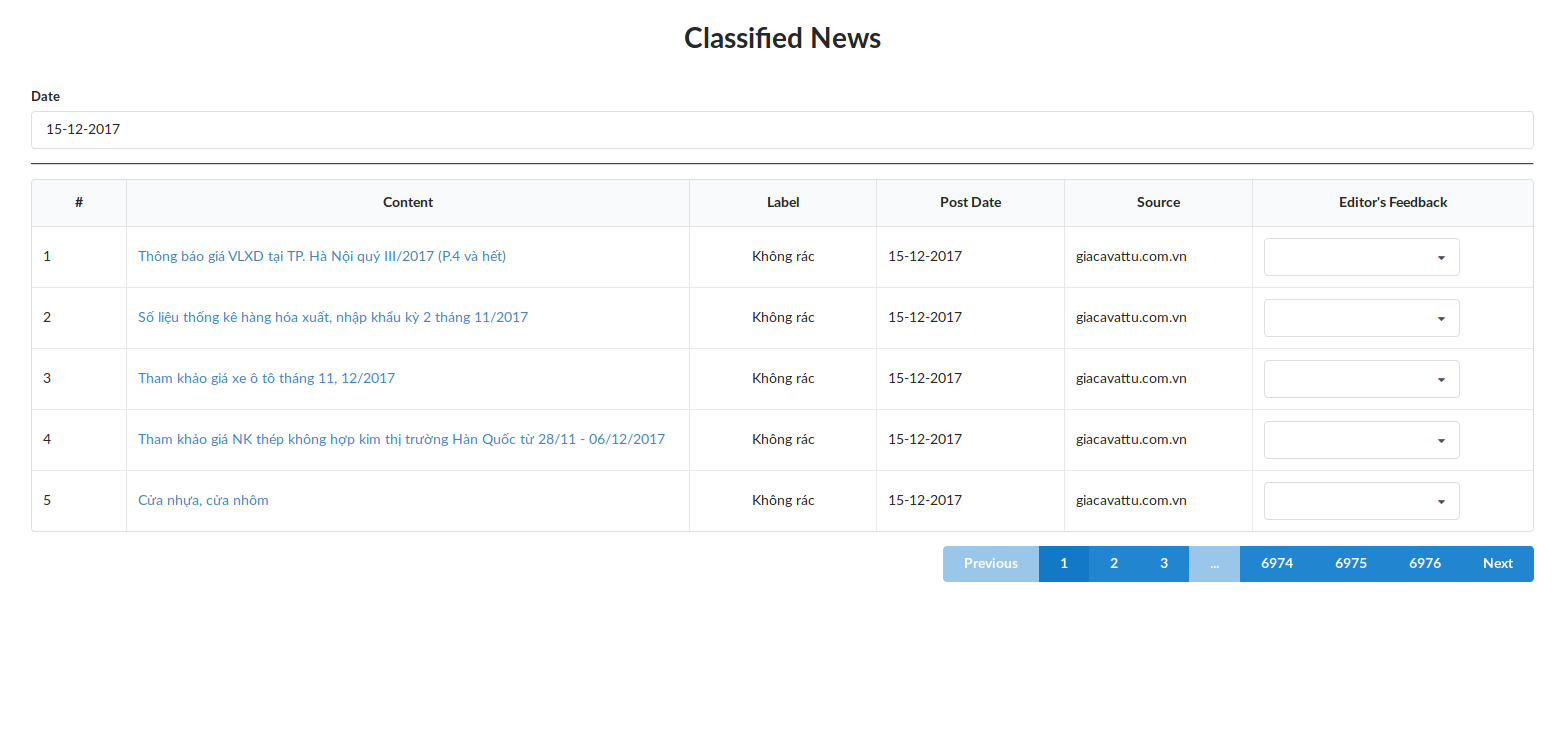
\includegraphics[width=1\linewidth]{Chapter3/Chapter3Figs/Classified.png}
	\caption{Giao diện danh sách tin đã phân lớp. Người dùng có thể chọn ngày để hiển thị tin và gửi phản hồi về nhãn của tin.}
	\label{fig:streaming}
\end{figure}

\begin{figure}[H]
	\centering
	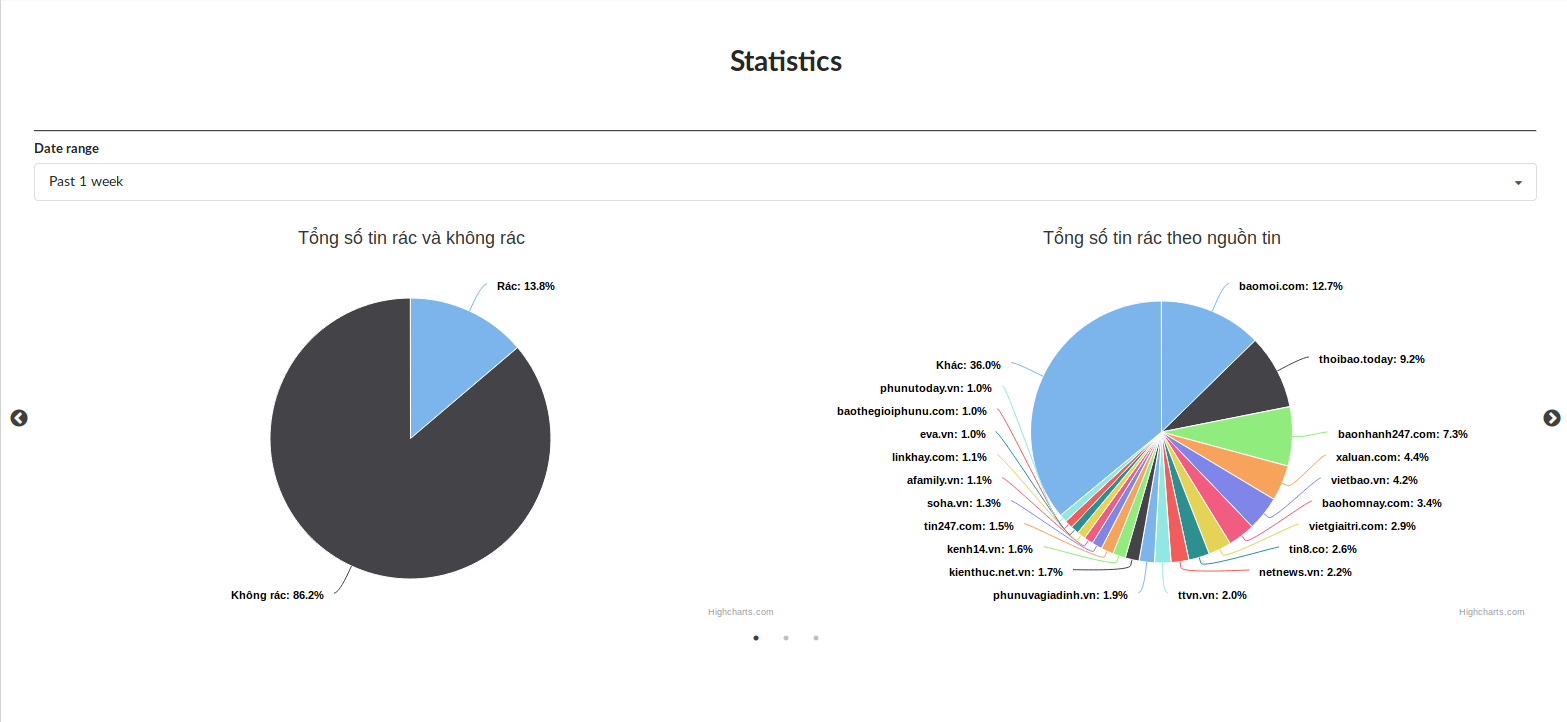
\includegraphics[width=0.96\linewidth]{Chapter3/Chapter3Figs/Chart1.png}
  \caption{Giao diện thống kê biểu đồ với hai biểu đồ. Biểu đồ thứ nhất thể hiện tổng số tin đã phân lớp phân theo nhãn "Rác" và "Không rác". Biểu đồ thứ hai thể hiện số lượng và tỉ lệ số lượng tin rác của mỗi nguồn tin so với tổng số tin rác và số tin rác của các nguồn tin khác (biểu đồ chỉ hiển thị top 20, nguồn tin có số lượng tin rác nhiều nhất)}
	\label{fig:streamingkeywords}
\end{figure}

\begin{figure}[H]
	\centering
	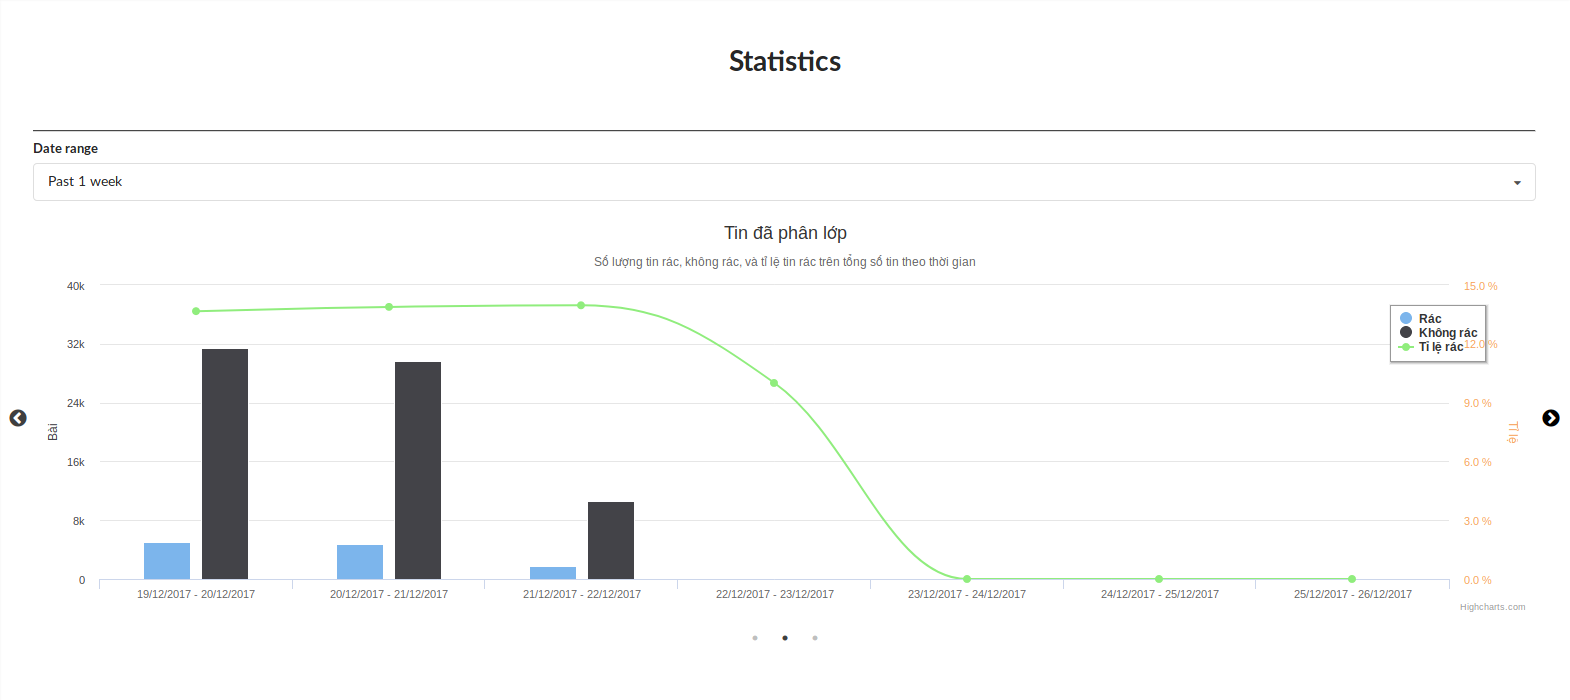
\includegraphics[width=0.96\linewidth]{Chapter3/Chapter3Figs/Chart2.png}
	\caption{Giao diện thống kê. Biểu đồ thể hiện số lượng tin "Rác" và "Không rác" và tỉ lệ tin "Rác" so với tổng số tin theo thời gian. Người dùng có thể chọn hiển thị số liệu thống kê trong hôm nay, 7 ngày trước, 30 ngày trước, hoặc 12 tháng trước }
	\label{fig:streamingkeywords}
\end{figure}

\begin{figure}[H]
	\centering
  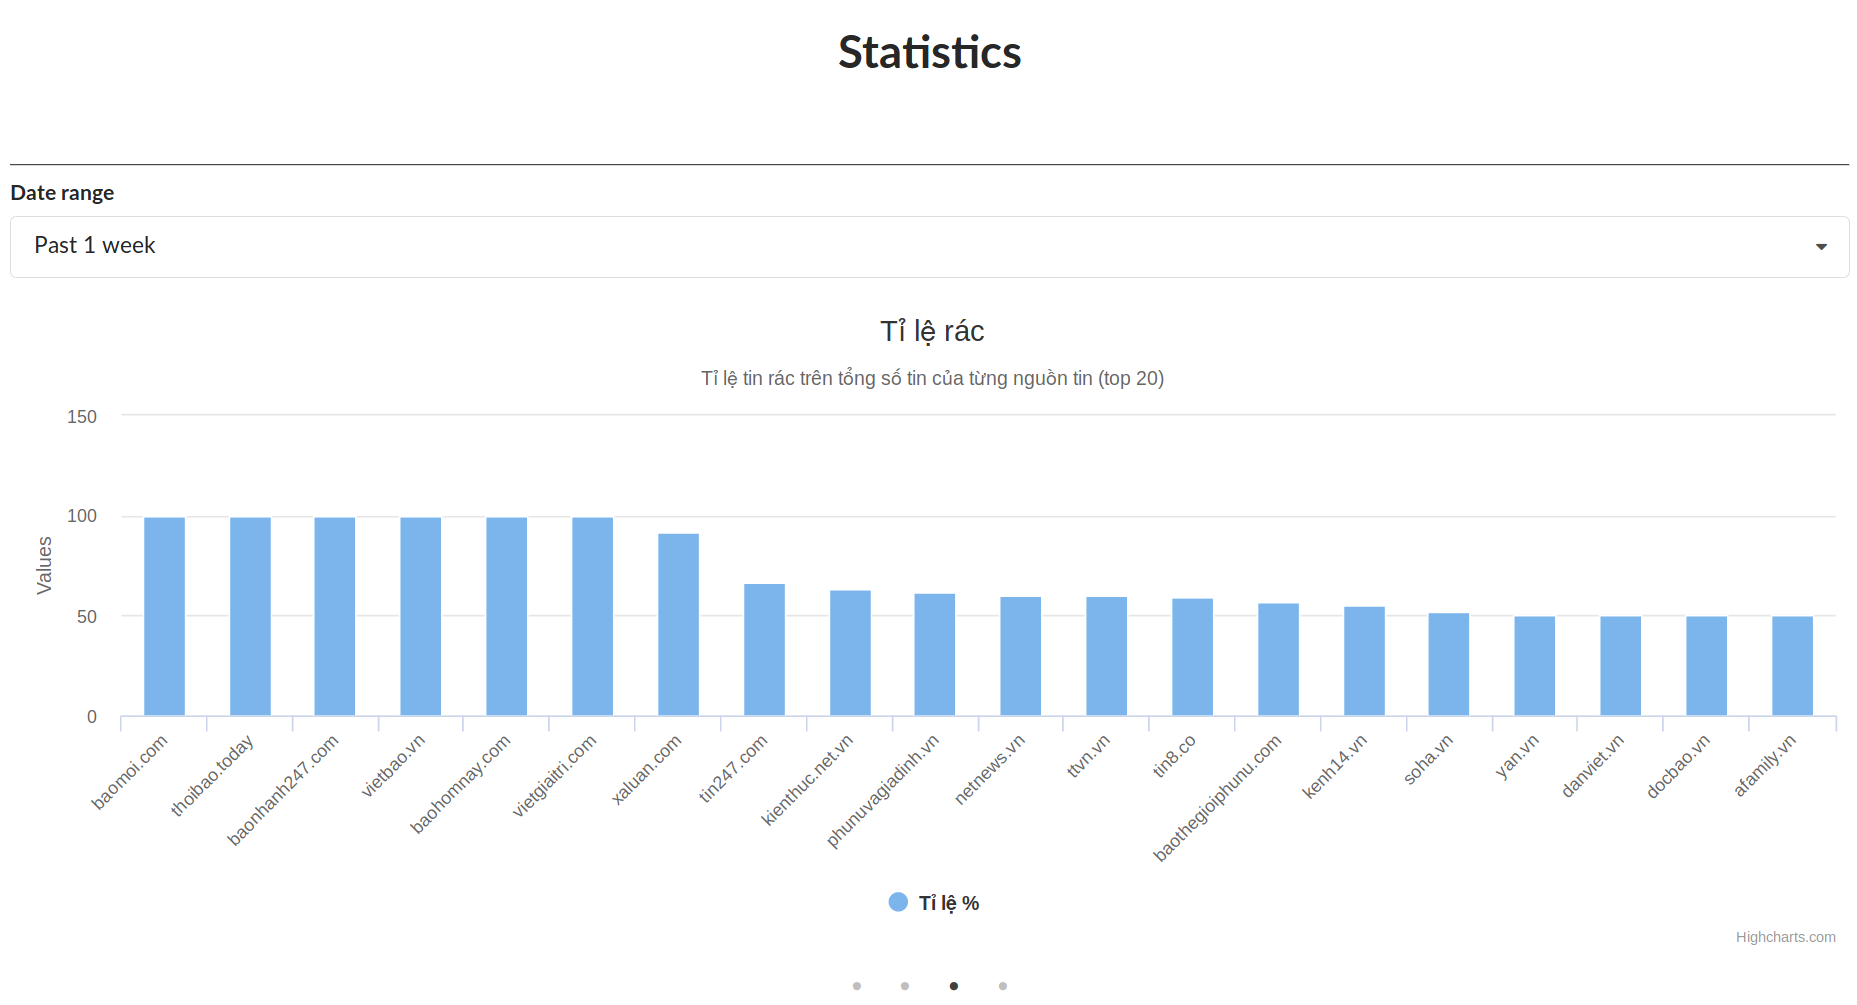
\includegraphics[width=0.96\linewidth]{Chapter3/Chapter3Figs/Chart3.png}
  \caption{Giao diện thống kê. Biểu đồ thể hiện tỉ lệ tin rác của một nguồn tin trên tổng số các tin của nguồn tin đó. Biểu đồ chỉ hiển thị top 20 nguồn tin với tỉ lệ lớn nhất và khác 0}
	\label{fig:streamingkeywords}
\end{figure}

\begin{figure}[H]
		\centering
	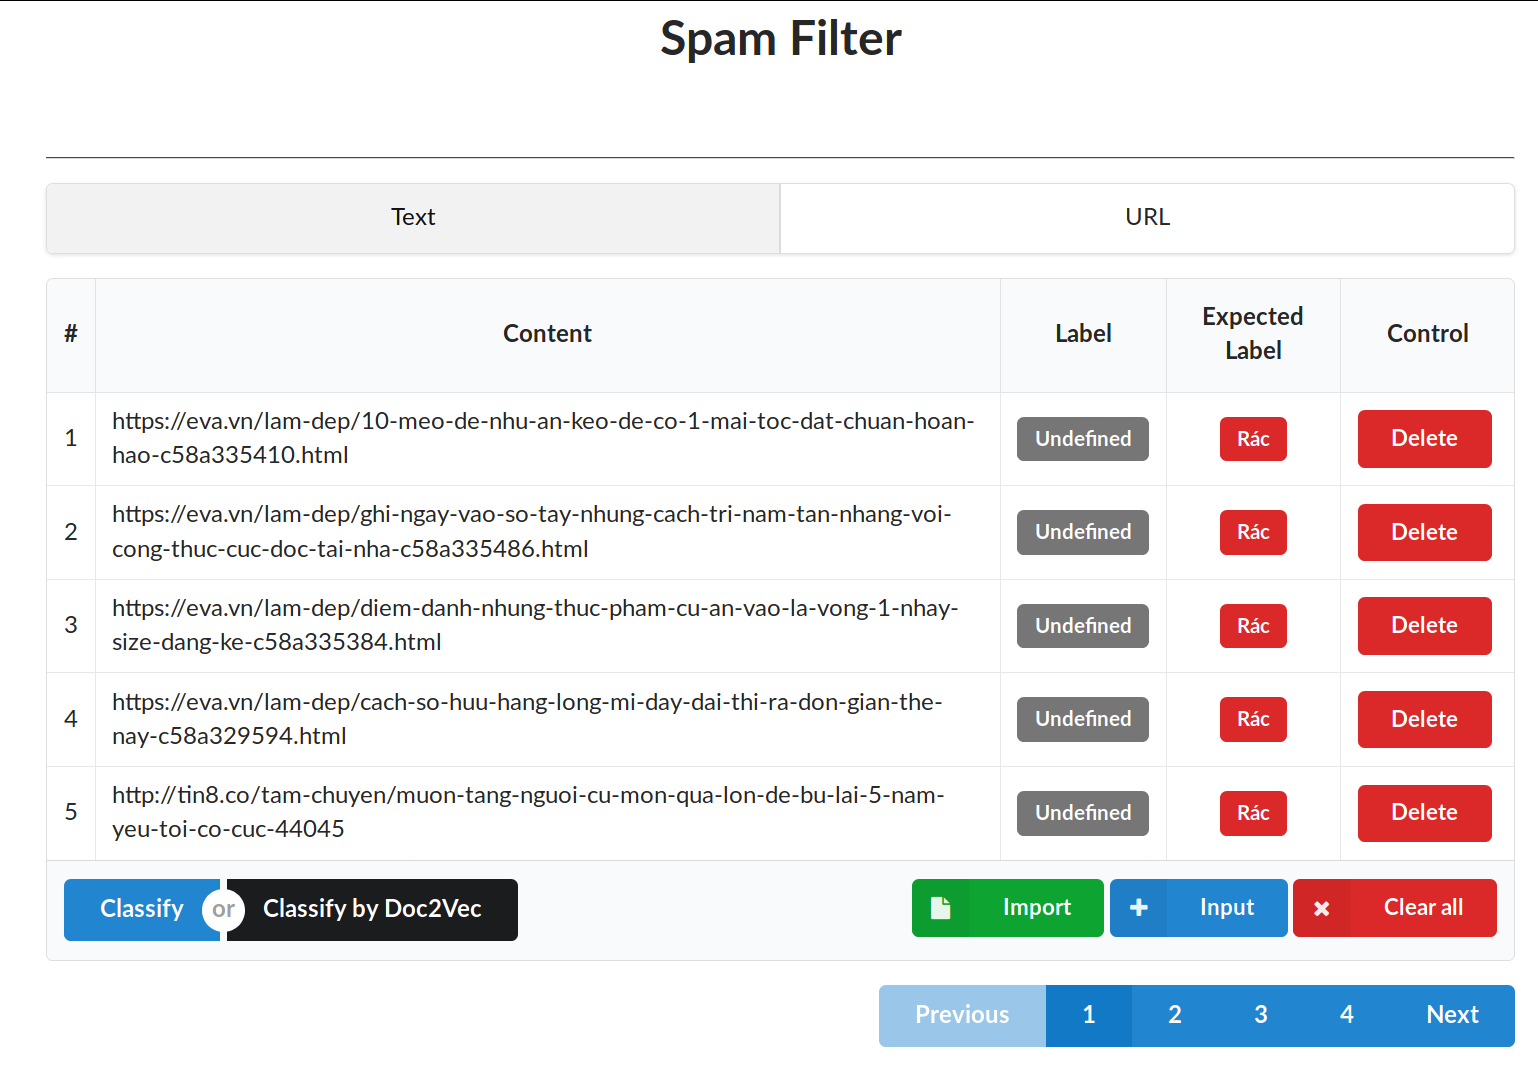
\includegraphics[width=0.96\linewidth]{Chapter3/Chapter3Figs/Filter.png}
	\caption{Giao diện bộ phân lớp tin tức. Người dùng có thể thực hiện phân lớp một cách thủ công bằng cách cho cho vào input là văn bản hoặc các đường dẫn đến các bài báo cần phân lớp, kèm theo là nhãn mà người dùng gán cho tin đó. Input có thể được truyền vào bằng cách nhập từ bàn phím hoặc truyền vào từ một file. Sao khi đã hoàn thành việc phân lớp, hệ thống sẽ trả về các nhãn tương ứng kèm theo độ chính xác của việc phân lớp và confusion matrix}
	\label{fig:startclustering}
\end{figure}

\section{Kết chương}
Chương này đã trình bày về các thành phần chính hệ thống, kiến trúc phân tầng, các hệ cơ sở dữ liệu được sử dụng và cách tổ chức, cùng một số kết quả cài đặt hệ thống.
\renewcommand\thefigure{4.\arabic{figure}} 
\setcounter{figure}{0}
\chapter{THỰC NGHIỆM VÀ ĐÁNH GIÁ}
\ifpdf
    \graphicspath{{Chapter4/Chapter4Figs/PNG/}{Chapter4/Chapter4Figs/PDF/}{Chapter4/Chapter4Figs/}}
\else
    \graphicspath{{Chapter4/Chapter4Figs/EPS/}{Chapter4/Chapter4Figs/}}
\fi

\section{Mở đầu}
Mục đích của chương này là trình bày kết quả huấn luyện các thuật toán phân lớp trên bộ dữ liệu thu thập được. Qua đó đánh giá, nhận định và so sánh các thuật toán phân lớp.

\section{Tổng quan về bộ dữ liệu}
Bộ dữ liệu gồm các bài viết từ các trang báo điện tử Việt Nam. Dữ liệu được lấy về từ cơ sở dữ liệu tin tức của công ty VCCorp\@. Dữ liệu thu thập được được sàn lọc thông qua một tập các từ khóa đã được định nghĩa trước.

Mỗi mẫu tin bao gồm các thông tin như sau: tựa đề tin, nội dung tin, mô tả tin, ngày đăng tin, và nguồn tin.

Bộ dữ liệu huấn luyện gồm 15,612 tin tiếng Việt, được thu thập và sàn lọc trong khoảng thời gian từ.

Dữ liệu thống kê cho tập dữ liệu sử dụng để train các model:
	\begin{table}[H]
		\centering
		\setlength\extrarowheight{3pt}
		\begin{tabular}{|l|l|l|}
			\hline
			Dữ liệu gán nhãn & Số lượng \\
			\hline
			Không rác   & 7331\\
			\hline
			Rác   & 8281\\
			\hline
			\hline
			Tổng   & 15612\\
			\hline
		\end{tabular}%
		\caption{Thống kê dữ liệu gán nhãn} \label{tab:table_4_1}%
	\end{table}
	\begin{table}[H]
		\centering
		\setlength\extrarowheight{3pt}
		\begin{tabular}{|l|l|l|}
			\hline
			Dữ liệu gán nhãn & Số lượng \\
			\hline
			Quảng cáo   & 4627\\
			\hline
			Chia sẻ   & 3279\\
			\hline
			Tuyển dụng   & 375\\
			\hline
			\hline
			Tổng   & 8281\\
			\hline
		\end{tabular}%
		\caption{Thống kê loại rác} \label{tab:table_4_2}%
	\end{table}
	\begin{table}[H]
%		\centering
		\setlength\extrarowheight{3pt}
		\begin{tabular}{|p{4cm}|p{10cm}|}
			\hline
			Chia sẻ      & thủ thuật, mẹo, tình cảm, chia tay, món ăn, ngon, tâm sự \\
			\hline
			Tuyển dụng   & việc làm, tuyển dụng, cộng tác viên, lao động \\ 
			\hline
			Quảng cáo & giảm giá, khuyển mãi, trúng thưởng \\
			\hline
		\end{tabular}%
		\caption{Danh sách từ khóa để thu thập dữ liệu}
		\label{tab:twitterkeywords}%
	\end{table}%

Bộ dữ liệu có thể được tải về từ địa chỉ:
\url{https://drive.google.com/open?id=1xZVBcaVtZAmQ4xU0KKPvB5ZRAUoKc2_v}

\section{Thiết lập thực nghiệm, cách đánh giá}
Sử dụng 3 thuật toán phân lớp: thuật toán Naive Bayes, thuật toán J48, thuật toán Support Vector Machine. 

Ta đánh giá và so sánh kết quả về thời gian xử lý và chất lượng phân lớp thông qua một số độ đo đã trình bày ở mục~\ref{sec:eval}: Precision, Recall, F-Measure, ROC Area, confusion matrix.

\section{Kết quả thực nghiệm}

	\subsection{Kết quả train model phân loại tin tức}
	Dưới đây là kết quả các thuật toán và kết quả của một số độ đo :
	\subsubsection{Kết quả dựa trên nội dung của tin của tập mẫu}
	\begin{table}[H]
		\centering
		\setlength\extrarowheight{3pt}
		\begin{tabular}{|l|l|l|}
			\hline
			Dữ liệu gán nhãn & Số lượng \\
			\hline
			Mẫu dữ liệu   & 15612\\
			\hline
			Số chiều   & 111363\\
			\hline
			Cross-validation:   & 10\\
			\hline
		\end{tabular}%
		\caption{Thông số cơ bản của tập train} \label{tab:table_4_3}%
	\end{table}
	\begin{table}[H]
		\centering
		\begin{tabular}{|l|l|l|}
			\hline
			Time build model(seconds): &            &          \\
			\hline
			SVM                        & NaiveBayes & J48      \\
			\hline
			382.85                     & 853.67     & 43530.21 \\
			\hline
		\end{tabular}
		\caption{Thời gian train model}
		\label{tab:table_4_4}
	\end{table}
	\begin{table}[H]
	\centering
	\rotatebox{90}{
		\begin{tabular}{|c|c|c|c|c|c|c|c|c|c|c|c|c|}
			\hline
			\multirow{2}{*}{Class} & \multicolumn{3}{c|}{Precision} & \multicolumn{3}{c|}{Recall} & \multicolumn{3}{c|}{F-Measure} & \multicolumn{3}{c|}{ROC Area} \\ \cline{2-13} 
			& J48     & SVM    & NaiveBayes  & J48    & SVM   & NaiveBayes & J48     & SVM    & NaiveBayes  & J48    & SVM    & NaiveBayes  \\ \hline
			Rác                    & 0.845   & 0.876  & 0.847       & 0.838  & 0.915 & 0.874      & 0.842   & 0.895  & 0.860       & 0.823  & 0.884  & 0.854       \\ \hline
			Tin                    & 0.819   & 0.898  & 0.852       & 0.827  & 0.854 & 0.821      & 0.823   & 0.876  & 0.836       & 0.823  & 0.884  & 0.871       \\ \hline
			& 0.832   & 0.887  & 0.849       & 0.833  & 0.886 & 0.849      & 0.832   & 0.886  & 0.849       & 0.823  & 0.884  & 0.862       \\ \hline
		\end{tabular}
		}
	\caption{Kết quả train model dựa trên một số độ đo}
	\label{tab:table_4_5}
	\end{table}%
	\subsubsection{Kết quả dựa trên tiêu đề của tin của tập mẫu}
	Dưới đây là kết quả các thuật toán và kết quả của một số độ đo :
	\begin{table}[H]
		\centering
		\setlength\extrarowheight{3pt}
		\begin{tabular}{|l|l|l|}
			\hline
			Dữ liệu gán nhãn & Số lượng \\
			\hline
			Mẫu dữ liệu   & 15612\\
			\hline
			Số chiều   & 15133\\
			\hline
			Cross-validation:   & 10\\
			\hline
		\end{tabular}%
		\caption{Thông số cơ bản của tập train} \label{tab:table_4_6}%
	\end{table}
	\begin{table}[H]
		\centering
		\begin{tabular}{|l|l|l|}
			\hline
			Time build model(seconds): &            &          \\
			\hline
			SVM                        & NaiveBayes & J48      \\
			\hline
			66.23                     & 130.78     & 5895.41	\\
			\hline
		\end{tabular}
		\caption{Thời gian train model}
		\label{tab:table_4_7}
	\end{table}
	\begin{table}[H]
		\centering
		\rotatebox{90}{
			\begin{tabular}{|c|c|c|c|c|c|c|c|c|c|c|c|c|}
				\hline
				\multirow{2}{*}{Class} & \multicolumn{3}{c|}{Precision} & \multicolumn{3}{c|}{Recall} & \multicolumn{3}{c|}{F-Measure} & \multicolumn{3}{c|}{ROC Area} \\ \cline{2-13} 
				& J48     & SVM    & NaiveBayes  & J48    & SVM   & NaiveBayes & J48     & SVM    & NaiveBayes  & J48    & SVM    & NaiveBayes  \\ \hline
				Rác                    & 0.845   & 0.876  & 0.847       & 0.838  & 0.915 & 0.874      & 0.842   & 0.895  & 0.860       & 0.823  & 0.884  & 0.854       \\ \hline
				Tin                    & 0.819   & 0.898  & 0.852       & 0.827  & 0.854 & 0.821      & 0.823   & 0.876  & 0.836       & 0.823  & 0.884  & 0.871       \\ \hline
				& 0.832   & 0.887  & 0.849       & 0.833  & 0.886 & 0.849      & 0.832   & 0.886  & 0.849       & 0.823  & 0.884  & 0.862       \\ \hline
			\end{tabular}
		}
		\caption{Kết quả train model dựa trên một số độ đo}
		\label{tab:table_4_8}
	\end{table}%
	\subsection{Kết quả train model phân loại loại tin rác}
	\begin{table}[H]
		\centering
		\setlength\extrarowheight{3pt}
		\begin{tabular}{|l|l|l|}
			\hline
			Dữ liệu gán nhãn & Số lượng \\
			\hline
			Mẫu dữ liệu   & 8281\\
			\hline
			Số chiều   & 9526\\
			\hline
			Cross-validation:   & 10\\
			\hline
		\end{tabular}%
		\caption{Thông số cơ bản của tập train} \label{tab:table_4_9}%
	\end{table}
	\begin{table}[H]
		\centering
		\begin{tabular}{|l|l|l|}
			\hline
			Time build model(seconds): &            &          \\
			\hline
			SVM                        & NaiveBayes & J48      \\
			\hline
			14.46                     & 19.39     & 590.78	\\
			\hline
		\end{tabular}
		\caption{Thời gian train model}
		\label{tab:table_4_10}
	\end{table}
	\begin{table}[H]
		\centering
		\rotatebox{90}{
			\begin{tabular}{|c|c|c|c|c|c|c|c|c|c|c|c|c|}
				\hline
				\multirow{2}{*}{Class} & \multicolumn{3}{c|}{Precision} & \multicolumn{3}{c|}{Recall} & \multicolumn{3}{c|}{F-Measure} & \multicolumn{3}{c|}{ROC Area} \\ \cline{2-13} 
				& NaiveBayes   & J48    & SVM    & NaiveBayes  & J48   & SVM   & NaiveBayes   & J48    & SVM    & NaiveBayes  & J48    & SVM    \\ \hline
				Chia sẻ                & 0.97         & 0.952  & 0.96   & 0.730       & 0.985 & 0.986 & 0.833        & 0.968  & 0.973  & 0.973       & 0.978  & 0.980  \\ \hline
				Quảng cáo              & 0.931        & 0.990  & 0.99   & 0.945       & 0.968 & 0.975 & 0.938        & 0.979  & 0.982  & 0.962       & 0.980  & 0.981  \\ \hline
				Tuyển dụng             & 0.335        & 0.989  & 1      & 0.992       & 0.952 & 0.955 & 0.5          & 0.970  & 0.977  & 0.954       & 0.987  & 0.977  \\ \hline
				& 0.919        & 0.975  & 0.979  & 0.862       & 0.974 & 0.979 & 0.877        & 0.974  & 0.979  & 0.966       & 0.980  & 0.981  \\ \hline
			\end{tabular}
		}
		\caption{Kết quả train model dựa trên một số độ đo}
		\label{tab:table_4_11}
	\end{table}%
\section{Nhận xét}
	\subsection{Nhận định về các thuật toán phân lớp cho bài toán}
	Dựa vào bảng~\ref{tab:table_4_5},~\ref{tab:table_4_8} và~\ref{tab:table_4_11}, ta thấy rằng với độ đo và tập dữ liệu mẫu, thuật toán Support Vector Machine cho kết quả tốt với mọi độ đo so với thuật toán Naive Bayes và J48.\\
	Dựa vào bảng~\ref{tab:table_4_4},~\ref{tab:table_4_7} và~\ref{tab:table_4_10}, ta thấy rằng thời gian để train model cho thuật toán Support Vector Machine tốn ít thời gian hơn thuật toán Naive Bayes và J48.
\section{Kết chương}
Qua các kết quả thử nghiệm, chương này đã thể hiện được một số tính chất của các thuật toán được đánh giá như thời gian train, một số độ đo thường dùng để đánh giá một hệ phân lớp. Ta thấy thuật toán SVM có thời gian train nhanh trong khi vẫn giữ được độ chính xác tốt so với thuật toán Naive Bayes và J48. Riêng thuật toán J48 có hạn chế về thời gian train quá lớn so với hai thuật toán còn lại.
\chapter*{\begin{center}KẾT LUẬN \\VÀ HƯỚNG PHÁT TRIỂN \end{center}}
\addcontentsline{toc}{chapter}{KẾT LUẬN VÀ HƯỚNG PHÁT TRIỂN}
\ifpdf
    \graphicspath{{Conclusions/ConclusionsFigs/PNG/}{Conclusions/ConclusionsFigs/PDF/}{Conclusions/ConclusionsFigs/}}
\else
    \graphicspath{{Conclusions/ConclusionsFigs/EPS/}{Conclusions/ConclusionsFigs/}}
\fi

\def\baselinestretch{1.66}

\section*{Kết quả đạt được}
%Viết lại chỗ này. Dan dat tu mục tiêu đề tài lúc đầu là gì? Cách tiếp cận và các nội dung cần thực hiện lúc đầu là gì? Chọn lựa phương pháp ra sao? Cái nào tốt? Tốt cái gì? Xấu cài gì? Tóm lại kết quả đạt được sau thời gian thực hiện đề tài lài gì? Phân loại (Kiến thức, Sản phẩm mềm: Bộ dữ liệu, Chương trình cài đặt các thuật toán ABC, Kết quả thực nghiệm đánh giá, so sánh các thuật toán ABC, hệ thống nhận biết tin nóng ... hiện điện trang khai sử dụng tại VCCorp), Liệt kê...


\addcontentsline{toc}{section}{Kết quả đạt được}
Mục tiêu chính của đề tài là xây dựng hệ thống phát hiện tin nóng để hỗ trợ biên tập viên trong việc viết bài. Một số nội dung thực hiện được đề ra ban đầu là: tìm hiểu bài toán liên quan, thu thập dữ liệu, cài đặt và đánh giá một số thuật toán, và xây dựng hệ thống. 

Sau quá trình nghiên cứu và thực hiện, khóa luận đã thu được một số kết quả sau:
	\begin{itemize}
		\item Kiến thức:
		\begin{itemize}
			\item Tìm hiểu về bài toán phát hiện tin tức, tin nóng trên dữ liệu từ mạng xã hội.
%			\item Tìm hiểu về các công ng
		\end{itemize}
		
		\item Sản phẩm:
		\begin{itemize}
			\item Thu thập bộ dữ liệu gồm các bài đăng tiếng Việt từ nguồn Twitter.
			\item Khảo sát và đánh giá các phương pháp phát hiện tin nóng dựa trên gom cụm: k-Nearest Neighbor, Boost Named Entity, Locality Sensitive Hashing.
			\item Xây dựng được hệ thống có khả năng nhận biết tin nóng, đang được triển khai tại công ty VCCorp.
		\end{itemize}
	\end{itemize}
%Với mục tiêu hỗ trợ biên tập viên nhanh chóng phát hiện tin nóng trên mạng xã hội Twitter, khóa luận đã đạt được một số kết quả nhất định như sau:
%	\begin{itemize}
%		\item Khảo sát và đánh giá các phương pháp phát hiện tin nóng: Nearest Neighbor, Boost Named Entity, Locality Sensitive Hashing.
%		\item Xây dựng được hệ thống có khả năng phát hiện sớm các tin tức đáng chú ý.
%	\end{itemize}

\section*{Hướng phát triển}
\addcontentsline{toc}{section}{Hướng phát triển}
Tuy hệ thống đạt được kết quả tương đối khá tốt trong việc phát hiện các sự kiện, cần cải thiện độ chính xác của thuật toán thông qua việc cân chỉnh kĩ hơn các thông số, đồng thời xem xét tìm hiểu thêm và so sánh với các phương pháp khác.

Trong tương lai hệ thống cần lấy thêm dữ liệu từ các nguồn khác như Facebook và các trang báo mạng để làm giàu nguồn tin. Thêm các chức năng tiện ích cho biên tập viên như thống kê dữ liệu tổng quát lẫn chi tiết, cung cấp cho biên tập viên nhiều góc nhìn về sự kiện hơn.

%Cải thiện model thu thập ý kiến btv
%Đóng gói thuật toán

\renewcommand{\bibname}{TÀI LIỆU THAM KHẢO} % changes default name Bibliography to References

\backmatter  


%\bibliographystyle{unsrtnat} % bibliography style
%\bibliographystyle{apa}
\bibliographystyle{unsrt}
%\bibliographystyle{Classes/plainnat} % bibliography style
%\bibliographystyle{Classes/IEEEtran} % bibliography style
%\bibliographystyle{Classes/splncs03} % bibliography style
%\bibliographystyle{Classes/jmb} % bibliography style

\bibliography{References/PhDResearch} % References file
\definecolor{dkgreen}{rgb}{0,0.6,0}
\definecolor{gray}{rgb}{0.5,0.5,0.5}
\definecolor{mauve}{rgb}{0.58,0,0.82}

\lstset{
	basicstyle=\ttfamily,
	frame=single, % adds a frame around the code
	xleftmargin=3.4pt,
	xrightmargin=3.4pt,	
	columns=flexible,
	showstringspaces=false,
	language=Java,
	numberstyle=\tiny\color{gray},
	keywordstyle=\color{blue},
	commentstyle=\color{dkgreen},
	stringstyle=\color{mauve},
	breaklines=true,
	breakatwhitespace=true,
	tabsize=3
}
\lstset{literate=
	{á}{{\'a}}1		{à}{{\`a}}1 	{ả}{{\h{a}}}1 	{ã}{{\~a}}1 	{ạ}{{\d{a}}}1
	{â}{{\^a}}1 	{ấ}{\'{\^a}}1 	{ầ}{\`{\^a}}1	{ẩ}{\h{\^a}}1	{ẫ}{\~{\^a}}1 	{ậ}{\d{\^a}}1
	{ă}{{\u{a}}}1	{ắ}{\'\u{a}}1	{ằ}{\`\u{a}}1	{ẳ}{\h\u{a}}1	{ẵ}{\~\u{a}}1	{ặ}{\d\u{a}}1	
	{é}{{\'e}}1		{è}{{\`e}}1		{ẻ}{{\h{e}}}1	{ẽ}{{\~e}}1		{ẹ}{{\d{e}}}1
	{ê}{{\^{e}}}1	{ế}{\'\^{e}}1	{ề}{\`{\^{e}}}1	{ể}{\h\^{e}}1	{ễ}{\~\^{e}}1	{ệ}{\d\^{e}}1
	{í}{{\'i}}1		{ì}{{\`i}}1		{ỉ}{{\h{i}}}1	{ĩ}{{\~i}}1		{ị}{{\d{i}}}1
	{ó}{{\'o}}1		{ò}{{\`o}}1		{ỏ}{{\h{o}}}1	{õ}{{\~o}}1		{ọ}{{\d{o}}}1
	{ơ}{{\ohorn}}1 	{ớ}{\'\ohorn}1	{ờ}{\`\ohorn}1	{ở}{\h\ohorn}1 	{ỡ}{\~\ohorn}1 	{ợ}{\d\ohorn}1
	{ô}{{\^o}}1 	{ố}{\'\^o}1		{ồ}{\`\^o}1		{ổ}{\h\^o}1 	{ỗ}{\~\^o}1 	{ộ}{\d\^o}1 	
	{ú}{{\'u}}1		{ù}{{\`u}}1		{ủ}{{\h{u}}}1	{ũ}{{\~u}}1		{ụ}{{\d{u}}}1
	{ư}{\uhorn}1 	{ứ}{\'\uhorn}1 	{ừ}{\`\uhorn}1 	{ử}{\h\uhorn}1 	{ữ}{\~\uhorn}1 	{ự}{\d\uhorn}1 
}
\chapter*{Phụ lục. Giới thiệu về thư viện Apache Lucene}

\section*{Giới thiệu}
\addcontentsline{toc}{chapter}{Phụ lục. Giới thiệu về thư viện Apache Lucene}
Truy hồi thông tin là một lĩnh vực nghiên cứu lớn nhắm giải quyết vấn đề tìm kiếm, lọc đường thông tin cần thiết, hữu ích từ lượng dữ liệu khổng lồ. Apache Lucene là một thư viện mã nguồn mở, được viết bằng Java và dùng để hỗ trợ giải bài toán này. Thư viện cung cấp khả năng đánh chỉ mục (index) trên dữ liệu và thực hiện tìm kiếm trên chỉ mục đó, cùng với các chức năng hỗ trợ khác.

Lucene lưu trữ dữ liệu ở dạng chỉ mục ngược (inverted index), cho phép tìm kiếm các đối tượng văn bản dựa trên từ khóa một cách nhanh chóng. Một đối tượng văn bản trong Lucene được gọi là Document. Mỗi Document có một hoặc nhiều Field, ứng với các thuộc tính của Document đó. Một bài viết hay một trang web có thể là một Document, với các Field như: tiêu đề, nội dung, tác giả, ngày đăng,...

Một số class chính của thư viện:
\begin{itemize}
	\item Analyzer và các class con: có nhiệm vụ phân tích dữ liệu văn bản thành những token/term trước khi ghi vào index. Một số class con như StandardAnalyzer, WhitespaceAnalyzer, SimpleAnalyzer, KeywordAnalyzer.
	\item IndexWriter: nhận luồng dữ liệu đã tokenize bằng Analyzer và ghi vào index.
	\item IndexReader, IndexSearcher: đọc và tìm kiếm trên index đã tạo từ trước, ngoài ra cung cấp các thông tin khác từ index như danh sách term, tần số của term trong một Document, trong toàn bộ dữ liệu.
	\item Query và các class con: dùng để xây dựng câu truy vấn và truyền vào IndexSearcher để thực hiện tìm kiếm. Một số class con như TermQuery, RangeQuery, Boolean Query. 
\end{itemize}

Hệ thống chủ yếu sử dụng Lucene hỗ trợ trong bước tiền xử lý dữ liệu, nhằm tính và biểu diễn các bài viết ở dạng vector tf-idf, thông qua các thông tin về tần số term trong index.

\section*{Sử dụng Lucene trong Java}
	\subsection*{Tạo IndexWriter}
	Để ghi dữ liệu vào Lucene index, ta cần tạo IndexWriter như sau:
		\begin{lstlisting}
	indexDirectory = FSDirectory.open(new File(indexDir)); 
	analyzer = new StandardAnalyzer(Version.LUCENE_36, Collections.emptySet());
	IndexWriterConfig config = new IndexWriterConfig(Version.LUCENE_36, analyzer);
	config.setOpenMode(OpenMode.CREATE);
	IndexWriter writer = new IndexWriter(indexDirectory, config);
		\end{lstlisting}
	\subsection*{Thêm một document vào index}
	Giả sử ta có một tweet với ID là "001", nội dung là "Tai nan kinh hoang khi xe tai mat phanh", dưới đây là cách tạo và thêm vào index document với 2 field tương ứng là "tweetID" và "tweetContent".
	
		\begin{lstlisting}
	Field tweetID = new Field("tweetID", "001", Field.Store.YES, Field.Index.NO);
	Field tweetContent = new Field("tweetContent", "Tai nan kinh hoang khi xe tai mat phanh", Field.Store.YES, Field.Index.ANALYZED, Field.TermVector.YES);				
	Document lucenceDocument = new Document();
	lucenceDocument.add(tweetID);
	lucenceDocument.add(tweetContent);
	writer.addDocument(luceneDocument);
		\end{lstlisting}
		
	\subsection*{Đọc dữ liệu từ index}
	Sau khi tạo index, ta có thể đọc thông tin trong index thông qua IndexReader hoặc IndexSearcher. 
		\begin{lstlisting}
	IndexReader reader = IndexReader.open(indexDir);
	IndexSearcher searcher = new IndexSearcher(reader);
		\end{lstlisting}
	
	Cách tính giá trị \textbf{idf} cho tất cả term trong field "tweetContent" trong bộ dữ liệu:
		\begin{lstlisting}	
	int docCount = reader.numDocs();
	TermEnum listOfTerms = reader.terms();
	TreeMap<String, Double> idfVector = new TreeMap<String, Double>();
	while (listOfTerms.next()) {
		String currentTerm = listOfTerms.term().text();
		int docFreq = searcher.docFreq(new Term("tweetContent", currentTerm));
		double idf = 1 + Math.log((double) docCount / docFreq);
		idfVector.put(currentTerm, idf);
	}
		\end{lstlisting}

	Cách tính vector tf-idf cho document thứ \textbf{i} trong index:	
%	Cách lấy danh sách term và tần số xuất hiện từng term trong một document có số thứ tự 0 (dùng để tính \textbf{tf} của từng term trong từng document):
		\begin{lstlisting}
	TermFreqVector tfv = reader.getTermFreqVector(i, "tweetContent");
	String[] termList = tfv.getTerms(); //list of terms in this document
	int[] termFreqList = tfv.getTermFrequencies();
	int totalTermCount = 0;
	LinkedHashMap<String, Double> tfidfVector = new LinkedHashMap<String, Double>();
	
	// calculate (total) term count in document i
	for (int temp : termFreqList) {
		totalTermCount += temp;
	}
	// loop through all term in doc i and calculate tfidf vector
	int uniqueTermCount = termList.length;
	for (int j = 0; j < uniqueTermCount; j++) {				
		if (termFreqList[j] != 0 && idfVector.containsKey(termList[j])){
			double tfidf = ((double)termFreqList[j] / totalTermCount)
			* idfVector.get(termList[j]);
			tfidfVector.put(termList[j], tfidf);
		}
	}
		\end{lstlisting}
		

\end{document}

